\documentclass{report}
\usepackage[utf8]{inputenc}
\usepackage{CJKutf8}
\usepackage{setspace}
\usepackage{enumitem}
\usepackage{amsmath}
\usepackage{chngcntr}
	\counterwithout{equation}{chapter}
\usepackage{hyperref}
\usepackage{graphicx}
	\graphicspath{{images/}}
\usepackage{float}
\usepackage{caption}
\usepackage[super,comma]{natbib}
\usepackage{geometry}
\usepackage{fancyhdr}
	\pagestyle{fancy}
	\fancyhead[R]{\leftmark}
	\fancyhead[L]{}
\renewcommand{\thefootnote}{\alph{footnote}}

\title{\LARGE{Enhancing interpretability of VAEs using biologically informed decoder for single-cell transcriptome analysis}
\vspace{20mm}}
\author{
	\Large{Masters Thesis}\\
	\\
	\Large{Presented to the Faculty of Biosciences}\\
	\Large{of the Ruprecht-Karls-Universität Heidelberg}}
\date{
	\vspace{30mm}
	\Large{Qian-Wu Liao}\\
	\Large{2022}
}

\setstretch{1.5}

\begin{document}
\maketitle

\thispagestyle{empty}
\noindent This Thesis was written at \textbf{Health Data Science Unit (HDSU) of Medical Faculty Heidelberg} at the Ruprecht-Karls-Universität Heidelberg in the period from \textbf{11.11.2021} to \textbf{25.05.2022} under the supervision of \textbf{PD Dr. Carl Herrmann} and \textbf{Daria Doncevic}.\vspace{5mm}\\
\\
1$\textsuperscript{th}$ Examiner: \textbf{Prof. Dr. Ursula Kummer}\\
Institute: \textbf{Centre for Organismal Studies (COS) Heidelberg}\\
\\
2$\textsuperscript{th}$ Examiner: \textbf{Prof. Dr. Julio Saez-Rodriguez}\\
Institute: \textbf{Institute for Computational Biomedicine of Universitätsklinikum Heidelberg}\vspace{2cm}\\
\\
\noindent I herewith declare that I wrote this Masters Thesis independently, under supervision, and that I used no other sources and aids than those indicated throughout the thesis.\vspace{1cm}\\
\\
Date \underline{\hspace{4cm}} \hspace{2cm} Signature \underline{\hspace{4cm}}


\chapter*{Abstract}
\addcontentsline{toc}{chapter}{Abstract}
Single-cell RNA sequencing (scRNA-seq) has revolutionized the analysis of transcriptomes for essentially any cell types and variational autoencoders (VAEs) have been proved to be a powerful tool for analyzing noisy single-cell transcriptomic data. However, typical VAE models provide little to no interpretability in their internal networks which are valuable for understanding biological mechanisms. To this end, this work aims at investigating the ability and various properties of two kinds of interpretable VAEs that either use the hard-coded decoder or use the regularized decoder where prior gene set annotations can be incorporated to guide the decoder wiring, which ends up modeling latent variables as the activity of distinctive gene modules. The interpretable latent space can then be used for many downstream studies such as cell type identities, cell states and differential activity analysis of different cell populations. We performed the benchmark studies using the published human adrenal medulla dataset to demonstrate the ability of these two types of interpretable models and indicate that they can be a complementary method to each other due to their unique attributes. Moreover, we also investigated some properties of these interpretable VAEs, such as the model reproducibility and the tolerance of the models to incorrect prior information, to provide more knowledge for further development and improvements.

\chapter*{Acknowledgements}
\addcontentsline{toc}{chapter}{Acknowledgements}
\begin{CJK*}{UTF8}{bsmi}
Firstly, I would like to express my deepest appreciation to my supervisors, Dr. Carl Herrmann and Daria Doncevic. Thank you for patiently imparting your knowledge to me and proactively guiding me through the journey of my thesis work. I enjoyed the time working with you very much. Secondly, I want to thank Prof. Dr. Ursula Kummer and Prof. Dr. Julio Saez-Rodriguez for being my thesis examiners. Thanks also to the people in Health Data Science Unit, Dr. Andres Quintero, Dr. Carlos Ramirez, Ana Luisa Costa, Youcheng Zhang and Lin Yang for any help and happy-happy moments during my thesis time. Thirdly, I want to thank Prof. Dr. Ju-Chien Cheng (鄭如茜 教授) and Dr. Jimmy Kuo (郭傑民 博士) for generously helping and guiding me towards my goal back in 2018 that was such a turning point of my life. Last but not least, I would like to thank my lovely family for always believing in and supporting me. Enriched by your energy, I will keep moving forward with faith in my life. (謝謝我最親愛的家人總是相信與支持我做的任何決定,在未來的路上我會帶著你們的能量與信念繼續朝我的目標前進。)
\end{CJK*}

\tableofcontents

\chapter*{List of abbreviations}
\addcontentsline{toc}{chapter}{List of abbreviations}
\newlist{abbrv}{itemize}{1}
\setlist[abbrv,1]{label=,labelwidth=1in,align=parleft,itemsep=0.1\baselineskip,leftmargin=!}
\begin{abbrv}
	\item[AE]	Autoencoder
	\item[AUC]	Area under the curve
	\item[BF]	Bayes factor
	\item[ChIP-seq]	Chromatin immunoprecipitation sequencing
	\item[GMV]	Gene module variable
	\item[GRN]	Gene regulatory network
	\item[IQR]	Interquartile range
	\item[KLD]	Kullback-Leibler divergence
	\item[PBMCs]	Peripheral blood mononuclear cells
	\item[PCC]	Pearson correlation coefficient
	\item[scRNA-seq]	Single-cell RNA sequencing
	\item[SCENIC]	Single-cell regulatory network inference and clustering
	\item[SCPs]	Schwann cell precursors
	\item[siRNA]	Small interfering RNA
	\item[TF]	Transcription factor
	\item[UMAP]	Uniform Manifold Approximation and Projection
	\item[VAE]	Variational autoencoder
	\item[VEGA]	VAE enhanced by gene annotations
\end{abbrv}


\chapter{Introduction}
\section{Single-cell RNA sequencing}
Recent advances in single-cell RNA sequencing (scRNA-seq) technologies\cite{Kolodziejczyk2015} have boosted many biological and clinical discoveries at an unprecedented resolution. Previously, sequencing technologies, such as bulk RNA-seq\cite{Emrich2007}, can only provide a gene expression profile of an entire sample containing thousands to millions of cells, revealing an overall state and biological traits of a whole organ or tissue. However, knowledge from a population of cells cannot represent that from an individual cell since biological signals of a minority of cells within a cell pool or slight differences in two cells of the same cell type may fail to be effectively detected\cite{Haque2017}, for example, malignant tumor cells within a tumor mass\cite{Tirosh2016} and individual T cells with highly diverse T cell receptors\cite{Stubbington2016}. To address this issue, scRNA-seq can be used to disentangle single cells from pooled cells, providing cellular heterogeneity that is valuable for many research focuses such as cellular traits, cellular responses to different scenarios and so on. In addition, data generated from scRNA-seq is also beneficial to gene regulatory networks (GRN) inferences in a data-driven way, providing context-specific GRNs which enables us to decipher functional cellular heterogeneity\cite{Haque2017}. Nevertheless, although scRNA-seq fulfills high-resolution transcriptomic analysis, it still has some challenges and limitations, such as drop-out events due to extremely low gene expression\cite{Ran2020}, batch effects between datasets from different measurements\cite{Tran2020} and so on, which complicates scRNA-seq data analysis\cite{Liu2016}. To extract meaningful biological information from high-dimensional noisy scRNA-seq data (i.e., dimensionality reduction), the selected computational method is critical. There are a variety of developed or developing computational methods used for data dimensionality reduction, e.g., for linear algorithms, principal component analysis\cite{Jolliffe2016} (PCA) and non-negative matrix factorization\cite{Quintero2020} (NMF). Compared to linear algorithms, nonlinear algorithms such as deep learning-based models have been proved to be a more advanced technique to learn more complex patterns from noisy transcriptomic data. Specifically, we focused on autoencoder-based models in our work.

\section{Autoencoder-based approaches}
Autoencoders\cite{Hinton2006} (AEs) have emerged as potent tools to tackle many different biological tasks such as dimensionality reduction of data\cite{Wang2018}, cell clustering\cite{Geddes2019} and data denoising\cite{Eraslan2019}. Compared to those methods that are limited by their linear nature (e.g., PCA), AEs are capable of learning more complex nonlinear patterns in single-cell transcriptomes. Generally, AEs consist of two parts: An encoder which can learn a nonlinear transformation projecting data from the high-dimensional input space to the lower-dimensional latent space (i.e., the representations of the input data) and a decoder which also learns a nonlinear transformation projecting the representations from the low-dimensional latent space back to the original high-dimensional input space\cite{Kleut2020} (Fig.\ref{fig:graphical_abstract_AE}). To optimize the quality of the information that the representations hold, AEs are trained end-to-end by minimizing the difference between the input data and the reconstructed data. Through this way, we can also turn dimensionality reduction tasks which are usually handled by unsupervised learning methods into supervised learning problems, which can potentially improve the accuracy of representations of input data. However, as previously mentioned, since single-cell transcriptomic data is usually very noisy and complex, it will be problematic if we want to use AEs as generative models due to their discrete latent space, leading to the poor generalizability. To be more concrete, the representations of all data points in the input data are vectors which are disjoint and non-continuous\cite{Kleut2020}, so nuances in input transcriptomic data may bring about unsatisfying reconstructed gene expression profiles. To this end, variational autoencoders\cite{Kingma2014} (VAEs) were developed. Instead of discrete latent vectors, VAEs map high-dimensional data to a probability distribution (e.g., a multivariate normal distribution) from which the lower-dimensional representations can be sampled (Fig.\ref{fig:graphical_abstract_VAE}), which makes the latent space more continuous and complete\cite{Kleut2020,Rocca2019}. VAEs have been demonstrated to work well for the probabilistic modeling of transcriptomic data in previous single-cell transcriptome studies such as scVI\cite{Lopez2018} and scGen\cite{Lotfollahi2019}. Even though the latent space of VAEs is modeled as a fairly complete and informative distribution, which enables VAEs to have the generative capacity and make accurate predictions, yet, it provides little to no interpretability that is crucial for understanding biological mechanisms. To gain more interpretability of internal networks, prior biological knowledge can be integrated into network structures. DCell\cite{Ma2018}, a deep interpretable neural network, has successfully embedded the hierarchies of molecular subsystems about cellular processes in the network architecture, which models not only functional outcomes but also the mechanisms resulting in these outcomes. To this end, the question is how VAEs can incorporate prior knowledge with network architectures to improve the model interpretability.\vspace{2mm}

\begin{figure}[h!]
    \centering
    \includegraphics[scale=0.60]{introduction/AE.png}
    \caption{\small{\textbf{Architecture of typical AE}}}
    \label{fig:graphical_abstract_AE}
\end{figure}

\begin{figure}[h!]
    \centering
    \includegraphics[scale=0.60]{introduction/VAE.png}
    \caption{\small{\textbf{Architecture of typical VAE}}}
    \label{fig:graphical_abstract_VAE}
\end{figure}

\section{Interpretable variational autoencoders}\label{introduction:model}
Inspired by f-scLVM\cite{Buettner2017} that uses prior gene set annotations to guide factor analysis and VAEs which use a factor model as a decoder\cite{Svensson2020}, a novel network architecture called VEGA (VAE enhanced by gene annotations) was proposed by Seninge et al. (2021), which consists of a two-layer nonlinear encoder and a single-layer masked linear decoder (Fig.\ref{fig:graphical_abstract}). Owing to the single-layer decoder where the latent variables (the representation of a single-cell transcriptome) directly connect to the output variables (the gene features), predefined gene set annotations either taken from databases (e.g., Reactome\cite{Gillespie2022} and MSigDB\cite{Liberzon2015}) or inferred using computational methods (e.g., SCENIC\cite{Aibar2017} and ARACNE\cite{Margolin2006}) can be used to guide the decoder wiring through a binary mask, which models the latent variables as biologically meaningful gene modules referred to as gene module variables (GMVs, see Methods \ref{methods:model}). To be more concrete, the values of gene expression of each cell are input to the encoder and encoded to the certain number of latent variables depending on the number of predefined gene modules provided. With the single-layer decoder, the connections between each latent variable and the genes in the output layer can be initiated by the prior gene set annotations, forcing the latent variables to be meaningful and interpretable by limiting them to certain corresponding sets of genes. Since any biological processes can be related to genes, it makes VEGA extremely flexible in terms of the specification of the connectivity of GMVs, which enables us to interpret single-cell transcriptomes from many other different viewpoints. Furthermore, since the decoder was designed as a linear factor model, the weights of a certain GMV to the gene reconstructions can be directly interpreted as the relationships between the GMV and the genes. Last, because different single-cell sequencing measurements always have technical noise and bias, VEGA can also incorporate batch information into the encoder and the latent space through one-hot encoding to combat batch effects, which was introduced in Lopez et al. (2018). Nevertheless, VEGA's hard-coded linear decoder leaves no room for further correcting or expanding existing prior knowledge which is usually incomplete or non-context-specific\cite{Seninge2021}. To have the decoder use prior knowledge more flexibly, instead of hard coding the decoder wiring, the L1 regularization technique\cite{Ng2004} can be employed on weights in the decoder to penalize those unannotated connections, which was introduced in Rybakov et al.(2020). Oppositely to the description above, predefined gene modules are used to pinpoint those GMV-gene relationships which are not included in the prior and the weights of those decoder connections will be penalized by gradually shrinking them to zero (see Methods \ref{methods:L1}). Using the regularized decoder enables the VAE to not only form the interpretable latent space but also potentially recover missing relationships between GMVs and genes in a data-driven fashion.\vspace{2mm}

\begin{figure}[h!]
    \centering
    \hspace*{-4.5mm}
    \includegraphics[scale=0.60]{graphical_abstract.png}
    \caption{\small{\textbf{Architecture of interpretable VAE} | The encoder is a two-layer nonlinear neural network which encodes high-dimensional input data to lower-dimensional representations and the representations are then modeled as a multivariate normal distributions in the latent space. The decoder is a single-layer factor model which attempts to reconstruct the representations sampled from the latent normal distribution to the original high-dimensional data. The connections between the latent variables (a representation of input data) and the output variables (input features) can be guided by prior knowledge through a binary mask. For scRNA-seq data analysis, the transcriptome of individual cells is the input to the model and predefined gene modules can be used to guide the decoder wiring. The solid lines in the decoder indicate there are relationships between GMVs and genes according to the prior used and the dashed lines indicate the opposite. There are two circumstances: (1) for the hard-coded decoder, the dashed connections always have zero-valued weights and (2) for the regularized decoder, the weights of the dashed connections are penalized through gradually shrinking them to zero. Moreover, batch information can also be incorporated into the encoder and the latent space through one-hot encoding to alleviate batch effects if needed. G above the matrices stands for gene and GM beside the binary matrix stands for gene module. GMVs represent gene module variables in the latent space.}}
    \label{fig:graphical_abstract}
\end{figure}

\section{Outline of our work}
In this work, we aimed at investigating the ability and various properties of interpretable VAEs that use the hard-coded decoder\cite{Seninge2021} and use the regularized decoder\cite{Rybakov2020}. Our work can be roughly split into three parts; firstly, to verify the availability of VEGA and better understand how exactly the model works, we reproduced the analyses of the well-studied PBMCs (peripheral blood mononuclear cells) dataset\cite{Kang2018} in the VEGA paper\cite{Seninge2021} using the Reactome pathways\cite{Jassal2020} as prior knowledge. Moreover, we sought to improve the model reproducibility which is important to the VEGA's main characteristic, interpretability, so we explored potential ways to boost the model reproducibility using the same dataset and prior knowledge. Secondly, we performed the benchmark studies on VEGA using the published human adrenal medulla dataset\cite{Jansky2021} and the SCENIC regulons\cite{Jansky2021} inferred from the same dataset as the prior. Note that we took advantage of the inferred TF activities of each adrenal medulla cell type group described in Jansky et al. (2021) as references for our benchmarks. Furthermore, we also employed the non-context-specific DoRothEA regulons\cite{Garcia-Alonso2019} as prior knowledge to observe the changes in the behavior of VEGA. Inspired by the results from the analyses of the adrenal medulla dataset\cite{Jansky2021} using the DoRothEA regulons as the prior, we investigated the tolerance of VEGA to incorrect information in prior knowledge by randomizing prior gene set annotations to different degrees. The last task we conducted in this section was testing the batch correction function\cite{Lopez2018} that is incorporated in VEGA. To do so, we took advantage of the human neuroblastoma dataset\cite{Jansky2021} which consists of 22 neuroblastoma samples and suffers from severe batch effects and the SCENIC regulons inferred from this tumor data as prior knowledge to see if VEGA is capable of screening out technical differences. In the last part of our work, we investigated the behavior and the ability of the interpretable VAE model using the regularized decoder by artificially modifying prior gene set annotations (i.e., artificial gene removal and addition) to see whether the regularized decoder manages to recover missing target genes or exclude non-biologically meaningful genes. Last, we studied the inference capacity of the regularized decoder by using the non-context-specific DoRothEA regulons as the prior, that is, we were interested in if the regularized decoder can infer more dataset-specific GRNs from general GRNs.


\chapter{Results}
\section{VEGA reproducibility}\label{results:reproducibility}
\subsection{Reproducing results in VEGA paper}
Firstly, to verify the ability and availability of VEGA\cite{Seninge2021}, we reproduced the analyses of the published PBMCs (peripheral blood mononuclear cells) dataset\cite{Kang2018} which consists of two groups of blood cells: Control cells and cells stimulated with interferon-$\beta$ (see Methods \ref{methods:data}). We wanted to see whether VEGA could recapitulate biological information in its interpretable latent space using the Reactome collection of pathways and processes\cite{Jassal2020} as prior knowledge to initiate the wiring of the decoder part of VEGA (see Methods \ref{methods:prior}). The hyperparameters used in this section are recorded in Appendix \ref{appendixA}. After the model training, we ran UMAP\cite{McInnes2020} on the VEGA embedding (see Methods \ref{methods:umap}). The results show that VEGA was capable of clustering cells into cell types and treatment conditions (Fig.\ref{fig:reproducibility}A;Appx.\ref{fig:reproducibility_appx}). Moreover, when specifically looking into GMV activities, we observed that the GMV representing the interferon-$\alpha$/$\beta$ signaling pathway separated stimulated and control cells, which is consistent with our result and previous studies\cite{Mazewski2020} (Fig.\ref{fig:reproducibility}B).

Next, we wanted to see if the differential GMV activities between two treatment conditions are statistically significant. For this, we performed differential activity analysis proposed by Seninge et al. (2021). Since each GMV is modeled into the posterior distribution, two mutually exclusive hypotheses can be formulated (i.e., a given GMV activity is higher in the stimulated group compared to the control group or the other way around) and the posterior probabilities of these hypotheses can be approximated through Monte Carlo sampling from the GMV distributions. Finally, a Bayes factor\cite{Kass1995,Held2018} (BF), the ratio of the hypothesis probabilities, can be used to determine the significantly differential GMV activities between two treatment conditions (see Methods \ref{methods:bf}). The volcano plot indicates that the activities of interest (interferon-$\alpha$/$\beta$ signaling and interferon signaling pathways) were significantly more active in the stimulated cells compared to the control cells ($|\textnormal{log}_e(\textnormal{BF})|>3$, Fig.\ref{fig:reproducibility}C). Together, these reproduced results confirm the interpretability of VEGA, enabling us to interpret gene expression data from the view of biological pathways and processes.\vspace{7mm}

\begin{figure}[h!]
    \centering
    \includegraphics[scale=0.47]{reproducibility/reproducibility.png}
    \caption{\small{\textbf{Reproduction of results in VEGA paper} | We reproduced the PBMCs analysis using the Reactome pathways as the prior. \textbf{(A)} The UMAP plot shows the model could cluster cells into cell types. \textbf{(B)} Since the dataset consists of control cells and cells stimulated by interferon-$\beta$, the interferon-$\alpha$/$\beta$ signaling pathway was of interest. The UMAP plot colored by activity levels of the GMV representing the interferon-$\alpha$/$\beta$ signaling pathway shows that stimulated and control cells were nicely separated and the stimulated cell group had a high level of the activity. \textbf{(C)} The x-axis and the y-axis indicate the significance level and the mean absolute difference of activity comparisons between two cell types. The volcano plot shows that interferon-$\alpha$/$\beta$ signaling and interferon signaling pathways were significantly more active in stimulated cells. We considered pathways to be significantly differentially activated if $|\textnormal{log}_e(\textnormal{BF})|>3$.}}
    \label{fig:reproducibility}
\end{figure}

\subsection{Using dropout layer in latent space stabilizes model reproducibility}\label{sec:reproducibility}
At the beginning of this work, we performed benchmarks for VEGA in an attempt to check the interpretability of the model and understand how exactly the model works. Specifically, we were interested in the stability of VEGA training since we found that some of the GMV activities in the latent space could be unrelated or even anticorrelated between two individual trained models on the same dataset (see Methods \ref{methods:stability}). Take the PBMCs dataset\cite{Kang2018} as an example using the same hyperparameters specified above (see Appendix \ref{appendixA}). We observed that the median of the correlations between two matching GMVs was 0.75 and some of them had negative correlations (Fig.\ref{fig:stability}A). We wondered if there are hyperparameters in control of the reproducibility of the GMV activities and then first dissected this question by investigating two novel hyperparameters introduced in VEGA: A dropout layer and additional fully connected nodes in the latent space. Note that the model used as the control was with $z\_dropout=0.5$ and $add\_nodes=1$ and we tuned one of these two hyperparameters each time to see the changes in the reproducibility. We found that, without employing a dropout layer in the latent space ($z\_dropout=0$), the median of the correlations dropped to 0.42 and the anticorrelated events became even worse (up to $-0.8$, Fig.\ref{fig:stability}A). There was no notable difference in the model reproducibility using a dropout rate of 0.3 and 0.5. On the other hand, we observed that with or without using additional nodes in the latent space did not significantly affect the reproducibility, where the median of the correlations slightly decreased from 0.72 to around 0.65 (Fig.\ref{fig:stability}A). Collectively, we suggest that the implementation of a dropout layer in the latent space have the effect of stabilizing the model reproducibility.

We next questioned whether the correlation coefficients of matching GMVs have any relationships with the numbers of genes in the output layer they connect to. We calculated the number of genes connected to each GMV and vice versa according to the Reactome prior knowledge and the considered highly variable genes (Appx.\ref{fig:stability_appx}). We display the results of using $z\_dropout=0.5$ and 0 (both with $add\_nodes=1$) for this task because we observed that employing a dropout layer in the latent space is a way to improve the model training stability. The results do not show any evident correlations between the reproducibility of GMVs and the numbers of genes which GMVs connect to (Fig.\ref{fig:stability}B,C). However, interestingly, we observed that additional nodes in the latent space always had a high correlation coefficient (0.99) when there was only one additional node employed, but had varied correlation coefficients ranging from -0.76 to 0.99 when more than one additional nodes were used (Fig.\ref{fig:stability}D). We infer that these additional nodes randomly shared learnable information with each other in different individual trained models since they all fully connected to genes in the output layer, leading to the poor characterization. Therefore, when we computed correlations, two corresponding latent variables might hold different information, leading to a low correlation coefficient. To this end, we propose the possible further work could be the investigation of whether gene programs having highly similar gene sets in prior information used to initiate the decoder wiring blur the reproducibility and the interpretability of GMVs because VEGA fails to model certain latent variables to specific biologically meaningful gene programs.\vspace{17mm}

\begin{figure}[h!]
    \centering
    \includegraphics[scale=0.70]{reproducibility/stability.png}
    \caption{\small{The caption is on the next page.}}
    \label{fig:stability}
\end{figure}

\newpage

\addtocounter{figure}{-1}
\begin{figure}[t!]
    \caption{\small{\textbf{Investigation of model training stability} | The method we used to measure the model training stability was computing Pearson correlation coefficients between two matching GMVs from two individual trained models using the same set of hyperparameters. We tuned two hyperparameters used in the latent space, one at a time: (1) \textit{z\_dropout} (the dropout rate) and \textit{add\_nodes} (the number of additional fully connected nodes) to investigate the changes in the training stability. Note that the correlations of the additional fully connected nodes were excluded from plot A, B and C. \textbf{(A)} The x-axis indicates the value of a hyperparameter and the y-axis indicates the correlation coefficient. The first boxplot ($z\_dropout=0.5$ and $add\_nodes=1$) was used as the control. The boxplots show that using a dropout layer in the latent space improved the stability of model training (green) and the number of additional nodes used in the latent space did not have influence on the training stability (purple). The box extends from the Q1 (25$\textsuperscript{th}$ percentile) to the Q3 (75$\textsuperscript{th}$ percentile) of data with the horizontal line inside denoting the median of data (Q2, 50$\textsuperscript{th}$ percentile). The whiskers extend from the box show the range of data (Q0, 0$\textsuperscript{th}$ percentile and Q4, 100$\textsuperscript{th}$ percentile) if all data points are within 1.5 * IQR (IQR = Q3 - Q1). Otherwise, the data points beyond the range are displayed as separate circles. IQR stands for interquartile range. \textbf{(B,C)} The x-axis indicates the number of genes each GMV connects to. The scatterplots show there were no evident correlations between the reproducibility of GMVs and the numbers of genes which GMVs connect to. PCC stands for Pearson correlation coefficient. \textbf{(D)} The x-axis indicates the number of additional fully connected nodes used in the latent space. The plot shows the reproducibility of some additional nodes could be very unstable when the number of additional nodes used was more than 1. The reason may be that the additional nodes randomly shared the learned information due to the same decoder wiring.}}
\end{figure}

\section{Performing benchmarks for VEGA}\label{results:benchmarks}
\subsection{TF activity analysis recapitulates adrenal medulla development}\label{sec:sparse_adm}
Secondly, we applied VEGA\cite{Seninge2021} to the published human adrenal medulla dataset\cite{Jansky2021} which consists of Schwann cell precursors (SCPs), chromaffin cells, neuroblasts and the other transient cells in the adrenal medulla from various stages of embryonic and fetal development (see Methods \ref{methods:data}). The UMAP\cite{McInnes2020} embedding of the gene expression space of the adrenal medulla cells shows the nice cell clustering and developmental trajectories where SCPs gave rise to chromaffin cells and neuroblasts through bridge and connecting progenitor cells\cite{Jansky2021} (Fig.\ref{fig:sparse_adm_scenic}A, see Methods \ref{methods:umap}). Moreover, the UMAP plot colored by samples reveals that the cell clustering was subject to biological differences between the cell types rather than technical differences between the samples (Appx.\ref{fig:sparse_adm_scenic_appx}A). As mentioned previously, owing to the flexibility of the GMV specification, we employed the SCENIC\cite{Aibar2017} regulons inferred from this human adrenal medulla dataset\cite{Jansky2021} as prior biological knowledge to guide the decoder wiring (see Methods \ref{methods:prior}). We wanted to see how capable VEGA is to capture TF activities at the single-cell level in its latent space, which can be used to conduct cell clustering and differential activity analysis. We first split the task into three parts where VEGA models were trained on (1) the dataset with the top 2000 highly variable genes, (2) the dataset with the whole gene features and (3) the dataset with only those genes connected to the GMVs according to the SCENIC regulons. The hyperparameters used in this task are recorded in Appendix \ref{appendixA}. After the VEGA training, we ran UMAP on the VEGA embeddings. Among these three trained models, all of them could nicely cluster cells into cell types (Fig.\ref{fig:sparse_adm_scenic}B;Appx.\ref{fig:sparse_adm_scenic_appx}B,C). Even so, the model trained on the dataset with the top 2000 highly variable genes best preserved the adrenal medulla development, which was thereby mainly used for the further work.

To investigate whether these GMVs truly represented certain SCENIC regulons, we performed differential activity analysis to statistically compare GMV activities between different cell types (see Methods \ref{methods:bf}). Note that the inferred TF activities of each adrenal medulla cell type group described in Jansky et al. (2021) were used as references for our benchmarks (Fig.\ref{fig:sparse_adm_scenic}C). The volcano plots show that VEGA precisely modeled the latent variables as the corresponding TFs in the prior because nearly all of the GMV (TF) activities of interest, except HES6, were averagely active in correct cell type groups (Fig.\ref{fig:sparse_adm_scenic}D) according to the references in Fig.\ref{fig:sparse_adm_scenic}C. For example, GATA3 and TFAP2B were found to have a high level of activities in neuroblasts and many members of the JUN/FOS TF family are associated with the chromaffin differentiation\cite{Jansky2021}. In the light of the ability of VEGA, those TFs which had significantly differential activities between different cell types but were not captured in Jansky et al. (2021), such as SREBF2 and E2F1 in neuroblasts compared to SCPs (Appx.\ref{fig:sparse_adm_scenic_appx}D), are extremely worth further investigation. However, we did not find any supporting biological evidence from previous studies for them in the context of healthy cells. Therefore, further work on verifying whether those significantly differential TF activities are biologically meaningful or just false positives is needed. Last but not least, the one additional fully connected node we used in the latent space was significantly active in neuroblasts and in chromaffin cells compared to SCPs, which indicates employing additional nodes helps capture extra information that is not explained in the prior (UNANNOTATED\_0 in Appx.\ref{fig:sparse_adm_scenic_appx}D).

\newpage

\begin{figure}[H]
    \centering
    \hspace*{-2mm}
    \includegraphics[scale=0.72]{SCENIC_sparse/adm_scenic_hvg_sparse.png}
    \caption{\small{\textbf{Benchmarks for VEGA} | We used the SCENIC regulons inferred from the human adrenal medulla dataset as prior knowledge to analyze TF activities of human adrenal medullary cells. \textbf{(A)} The UMAP embedding of the gene expression space shows the clear cell clustering and the developmental trajectories of the adrenal medulla. \textbf{(B)} The UMAP embedding of the VEGA latent space shows that the model could cluster cells into cell types and preserve the developmental trajectories. Note that the model were trained on the dataset with the top 2000 highly variable genes and we removed 23 SCENIC regulons from the prior, whose target genes did not overlap with any considered gene features, i.e., there would be no connections between these 23 GMVs and the genes in the output layer. \textbf{(C)} The inferred TF activities of each cell type group from Jansky et al. (2021) were used as references for our TF differential activity analysis. Firstly, the TF activities in individual cells were inferred using SCENIC and for each TF, the activities across cells were discretized into two levels (active or inactive) using k-means clustering. Finally, the TF activities of each cell type group were determined by computing the fraction of cells whose TF states were active in each cell type. \textbf{(D)} The x-axis and the y-axis indicate the significance level and the mean absolute difference of activity comparisons between two cell types. The volcano plots show that nearly all of the TF activities of interest, except HES6 (colored in green), were averagely active in correct cell type groups. We considered TFs to be significantly differentially activated if $|\textnormal{log}_e(\textnormal{BF})|>3$.}}
    \label{fig:sparse_adm_scenic}
\end{figure}

\newpage

\subsection{Hard-coded decoder leaves little freedom for further inferences}
Next, instead of using the dataset-specific prior to initiate the decoder wiring, we employed the DoRothEA\cite{Garcia-Alonso2019} regulons which is not context-specific to investigate the behavior of VEGA (see Methods \ref{methods:prior}). Of note, the hyperparameters used in this task are the same as Section \ref{sec:sparse_adm}, which is recorded in Appendix \ref{appendixA}. After the model training, we ran UMAP on the VEGA embedding. The result shows that VEGA was still able to cluster cells into cell types and also exhibit the developmental trajectories of the human adrenal medulla (Fig.\ref{fig:sparse_adm_dorothea_hvg}A). However, when we looked into the differential activity analysis results, we observed that VEGA using the general prior knowledge could not faithfully reflect the correct activations of TF activities in certain cell types anymore (Fig.\ref{fig:sparse_adm_dorothea_hvg}B). The differential activity analysis results took Fig.\ref{fig:sparse_adm_scenic}C as references. Although nearly all of the significantly differential TF activities, except CUX1, were correctly presented in the corresponding cell types, a majority of TF activities could not be captured or were even falsely predicted by VEGA (e.g., HIVEP3, JUNB, JUND and so on). We then checked the overlaps of the target genes between the DoRothEA and the SCENIC regulons and found that all target gene sets hardly overlap with each other (Table \ref{table:dorothea_scenic_outline}). Collectively, these results indicate that VEGA has limited freedom to further make inferences beyond the prior and fails to provide the interpretability in the latent space when prior knowledge used is not context-specific. Given that we still obtained such the clear clustering of the adrenal medullary cells, we reasoned that the compressed information that the VEGA latent variables hold can be extracted from the expression data with any decoder settings, but just the learned information will be randomly distributed in the latent space if the decoder wiring is biologically meaningless, which means the model loses its interpretability. This hypothesis will be corroborated in the next section.

\newpage

\begin{figure}[h!]
    \centering
    \hspace*{-5mm}
    \includegraphics[scale=0.76]{DoRothEA_sparse/adm_dorothea_hvg.png}
    \caption{\small{\textbf{Observations of VEGA using general regulons as prior knowledge} | We used the DoRothEA regulons which is not context-specific as the prior to investigate the changes in the model interpretability. \textbf{(A)} The UMAP plot shows the model could still cluster cells into cell types and preserve the developmental trajectories of the adrenal medulla. Note that we removed 19 DoRothEA regulons from the prior, whose target genes did not overlap with any considered gene features. \textbf{(B)} The x-axis and the y-axis indicate the significance level and the mean absolute difference of activity comparisons between two cell types. Note that the differential activity analysis results took Fig.\ref{fig:sparse_adm_scenic}C as references. The volcano plots show that even though nearly all the significantly differential TF activities, except CUX1 (colored in green), were correctly predicted, a majority of TF activities could not be captured or were even wrongly predicted (e.g., HIVEP3, JUNB and JUND) by the model. We considered TFs to be significantly differentially activated if $|\textnormal{log}_e(\textnormal{BF})|>3$.}}
    \label{fig:sparse_adm_dorothea_hvg}
\end{figure}

\begin{table}[h!]
    \begin{center}
        \captionsetup{width=.77\textwidth}
        \caption{\small{\textbf{Outline of DoRothEA and SCENIC regulons of interest} | Confidence levels are of DoRothEA, ranging from A (most confident) to E (least confident) depending on the amount of supporting biological evidence.}}
        \label{table:dorothea_scenic_outline}
        \begin{tabular}{|c|c|c|c|c|c|}
        \hline
        & \textbf{\small{Confidence}} & \textbf{\small{Gene set size}} & & \textbf{\small{Overlapping of}}\\
        \textbf{\small{TF}} & \textbf{\small{level}} & \textbf{\small{-DoRothEA-}} & \textbf{\small{-SCENIC-}} & \textbf{\small{target genes}}\\
        \hline
        \small{ALX3} & \small{E} & \small{385} & \small{101} & \small{4}\\
        \hline
        \small{ATF3} & \small{C} & \small{50} & \small{970} & \small{8}\\
        \hline
        \small{BHLHE40} & \small{C} & \small{58} & \small{633} & \small{5}\\
        \hline
        \small{CREM} & \small{C} & \small{52} & \small{1715} & \small{24}\\
        \hline
        \small{CUX1} & \small{C} & \small{41} & \small{617} & \small{5}\\
        \hline
        \small{EGR1} & \small{A} & \small{124} & \small{299} & \small{5}\\
        \hline
        \small{EGR4} & \small{E} & \small{476} & \small{62} & \small{4}\\
        \hline
        \small{ETS1} & \small{A} & \small{145} & \small{868} & \small{6}\\
        \hline
        \small{FOS} & \small{A} & \small{90} & \small{1071} & \small{10}\\
        \hline
        \small{FOSL2} & \small{A} & \small{10} & \small{1557} & \small{1}\\
        \hline
        \small{FOXO1} & \small{A} & \small{43} & \small{396} & \small{4}\\
        \hline
        \small{GATA3} & \small{A} & \small{73} & \small{543} & \small{1}\\
        \hline
        \small{HES6} & \small{E} & \small{199} & \small{202} & \small{4}\\
        \hline
        \small{HIVEP3} & \small{E} & \small{192} & \small{13} & \small{0}\\
        \hline
        \small{JUN} & \small{A} & \small{121} & \small{1975} & \small{19}\\
        \hline
        \small{JUNB} & \small{C} & \small{52} & \small{673} & \small{3}\\
        \hline
        \small{JUND} & \small{A} & \small{19} & \small{3470} & \small{3}\\
        \hline
        \small{NFATC1} & \small{C} & \small{35} & \small{120} & \small{0}\\
        \hline
        \small{NFIL3} & \small{D} & \small{11} & \small{252} & \small{0}\\
        \hline
        \small{NR2F2} & \small{A} & \small{18} & \small{287} & \small{0}\\
        \hline
        \small{SOX10} & \small{A} & \small{16} & \small{285} & \small{3}\\
        \hline
        \small{SIX11} & \small{C} & \small{29} & \small{161} & \small{1}\\
        \hline
        \small{SOX13} & \small{C} & \small{42} & \small{14} & \small{0}\\
        \hline
        \small{SOX2} & \small{A} & \small{10} & \small{168} & \small{0}\\
        \hline
        \small{SOX5} & \small{E} & \small{875} & \small{160} & \small{29}\\
        \hline
        \small{TFAP2B} & \small{E} & \small{796} & \small{984} & \small{55}\\
        \hline
        \end{tabular}
    \end{center}
\end{table}

\subsection{Randomizing predefined gene sets breaks model interpretability}
To scrutinize the importance of prior biological knowledge in terms of the interpretability of the VEGA latent space, we randomized the aforementioned SCENIC regulons inferred from the human adrenal medulla dataset\cite{Jansky2021} on varied levels (from 10\% to 90\%) and trained VEGA using them as the prior to see the changes in the interpretability (see Methods \ref{methods:randomization}). Of note, the set of hyperparameters used in this task is the same as Section \ref{sec:sparse_adm}, which is recorded in Appendix \ref{appendixA}. The UMAP embeddings of the latent spaces show that the models could cluster cells into cell types and retain the developmental trajectories no matter how randomized the \textit{a priori} defined gene sets were (Fig.\ref{fig:sparse_adm_rand_hvg}A). This result is theoretically expected because the compressed information that the VEGA latent variables hold mainly depends on the encoder part. The latent variables should in principle be able to learn the learnable variation in the gene expression data with any decoder settings. However, randomizing the predefined gene sets affected the VEGA interpretability to different degrees depending on the level of randomization. The models could preserve the interpretability when slightly randomized gene sets (up to 30\%) were used as the prior, which indicates little incorrect information in prior knowledge is tolerable (Fig.\ref{fig:sparse_adm_rand_hvg2};Appx.\ref{fig:sparse_adm_rand_hvg_appx}). From 40\% randomization, the models started making some obvious mistakes. For example, SOX11 has been found having high TF activities in neuroblasts, many members of the JUN TF family are associated with the chromaffin differentiation and FOXO1 has higher TF activities in SCPs compared to neuroblasts\cite{Jansky2021} (Fig.\ref{fig:sparse_adm_rand_hvg2};Appx.\ref{fig:sparse_adm_rand_hvg_appx}). These previous findings could not be presented by the corresponding GMVs for differential activity tests when the prior knowledge was greatly disorganized. Finally, when 90\% of target genes in the prior were shuffled, most of the GMVs could not faithfully reflect differential TF activities in different cell types anymore (Fig.\ref{fig:sparse_adm_rand_hvg2}). Of note, the differential activity analysis results took Fig.\ref{fig:sparse_adm_scenic}C as references.

Furthermore, we looked into the learning curves of VEGA which used these different levels of randomized gene sets as prior knowledge. We observed that the efficiency of the model training was highly related to the correctness of the prior knowledge, where the training loss dropped more rapidly when less randomized predefined gene sets were provided (Fig.\ref{fig:sparse_adm_rand_hvg}B). To be more concretely, simulating the decoder wiring as real gene regulatory networks (GRNs) helps VEGA discern relationships between TFs and genes, resulting in more efficient learning. For predictive performance, the validation loss reveals that the models trained using the original and up to 20\% randomized gene sets outperformed the other models trained using more than 20\% randomized gene sets and there was no apparent difference among the original prior, 10\% and 20\% randomized gene sets, which implies VEGA should be able to tolerate a bit of wrong information in the prior knowledge (Fig.\ref{fig:sparse_adm_rand_hvg}C). This finding is in line with our earlier differential activity test results, showing the models' interpretability could be preserved when the gene sets were mildly randomized (Fig.\ref{fig:sparse_adm_rand_hvg2}). To sum up, correct prior knowledge is important for VEGA to keep the interpretability and generate accurate inferences. Slightly wrong prior knowledge is acceptable but when the prior is incorrect to the certain degree, VEGA starts losing its interpretability since the hard-coded linear decoder leaves no room for correcting prior knowledge\cite{Seninge2021}.

\newpage

\begin{figure}[H]
    \centering
    \includegraphics[scale=0.72]{SCENIC_sparse/adm_rand_hvg.png}
    \caption{\small{\textbf{Investigation of model behavior by using disorganized prior} | We randomized the SCENIC regulons inferred from the human adrenal medulla data to different degrees (10\% - 90\%) to investigate the changes in the model behavior. \textbf{(A)} The UMAP plots show that the models could cluster cells into cell types and preserve the adrenal medulla developmental trajectories no matter how randomized the prior was, which corroborates VEGA is able to learn variation in gene expression data with any decoder settings. Note that we removed the same 23 SCENIC regulons from the prior, whose target genes did not overlap with any considered gene features from all versions of the prior knowledge. Rand indicates the degree of randomization of the prior. \textbf{(B,C)} The x-axis indicates the epoch of model training and the y-axis indicates the training and the validation loss. The loss curves show that the training efficiency was highly related to the correctness of the prior (see plot B) and the model could tolerate little wrong information in the prior (up to 20\% randomization, see plot C). Ori represents the original prior and Rand represents the randomized prior to different degrees.}}
    \label{fig:sparse_adm_rand_hvg}
\end{figure}

\newpage

\begin{figure}[H]
    \centering
    \hspace*{-10mm}
    \includegraphics[scale=0.8]{SCENIC_sparse/adm_rand_hvg2.png}
    \caption{\small{The caption is on the next page.}}
    \label{fig:sparse_adm_rand_hvg2}
\end{figure}

\addtocounter{figure}{-1}
\begin{figure}[h!]
    \caption{\small{\textbf{Changes in model interpretability when randomizing prior to different degrees} | The x-axis and the y-axis indicate the significance level and the mean absolute difference of GMV activity comparisons between two cell types. Note that the differential activity analysis results took Fig.\ref{fig:sparse_adm_scenic}C as references. The volcano plots show that the model kept the interpretability when the prior was 10\% randomized, made some obvious mistakes (TFs colored in green) when the prior was 40\% and 70\% randomized and failed to capture most of the TFs of interest when the prior was 90\% randomized. Rand indicates the degree of randomization of the prior. We considered TFs to be significantly differentially activated if $|\textnormal{log}_e(\textnormal{BF})|>3$.}}
\end{figure}

\subsection{Incorporating batch annotations in model combats batch effects}
Deep generative models taking batch information into account have been demonstrated to have the ability to combat batch effects which frequently occur in single-cell transcriptome measurements\cite{Lopez2018}. VEGA, as an interpretable VAE, can take advantage of this technique and incorporate batch annotations in the encoder and the latent space (see Methods \ref{methods:model}). To test the function of batch correction of VEGA, we used the human neuroblastoma dataset\cite{Jansky2021} which consists of 22 neuroblastoma samples and suffers from severe batch effects even though the data integration was performed (see Methods \ref{methods:data}). The UMAP embedding of the gene expression space clearly shows that cells were clustered mainly due to technical differences between the samples rather than biological differences between the cell types (Fig.\ref{fig:sparse_nb_batch}A). To remove technical confounders, we incorporated the batch annotations of the considered dataset during model training. Of note, the SCENIC regulons inferred from this human neuroblastoma dataset\cite{Jansky2021} were used as prior knowledge and the hyperparameters used in this task can be found in Appendix \ref{appendixA}. After the model training, we ran UMAP on the VEGA embedding. The results show that cells from the different samples were nicely blended and also clustered into cell types, which indicates the model was able to distinguish biological variation from technical variation when the batch information was provided (Fig.\ref{fig:sparse_nb_batch}B). We also trained VEGA with all the same settings except incorporating the batch information as the contrast. The results did not differ much from the UMAP plot of the gene expression space (Fig.\ref{fig:sparse_nb_batch}A), which still had strong batch effects (Appx.\ref{fig:sparse_nb_batch_appx}). Collectively, VEGA incorporating batch information in the encoder and the latent space can effectively alleviate batch effects and provide biologically meaningful representations of combined data. This is an exciting application because we can employ the same model to carry out not only data analysis but also data integration if needed, making the whole analysis procedure more consistent.

\begin{figure}[h!]
    \centering
    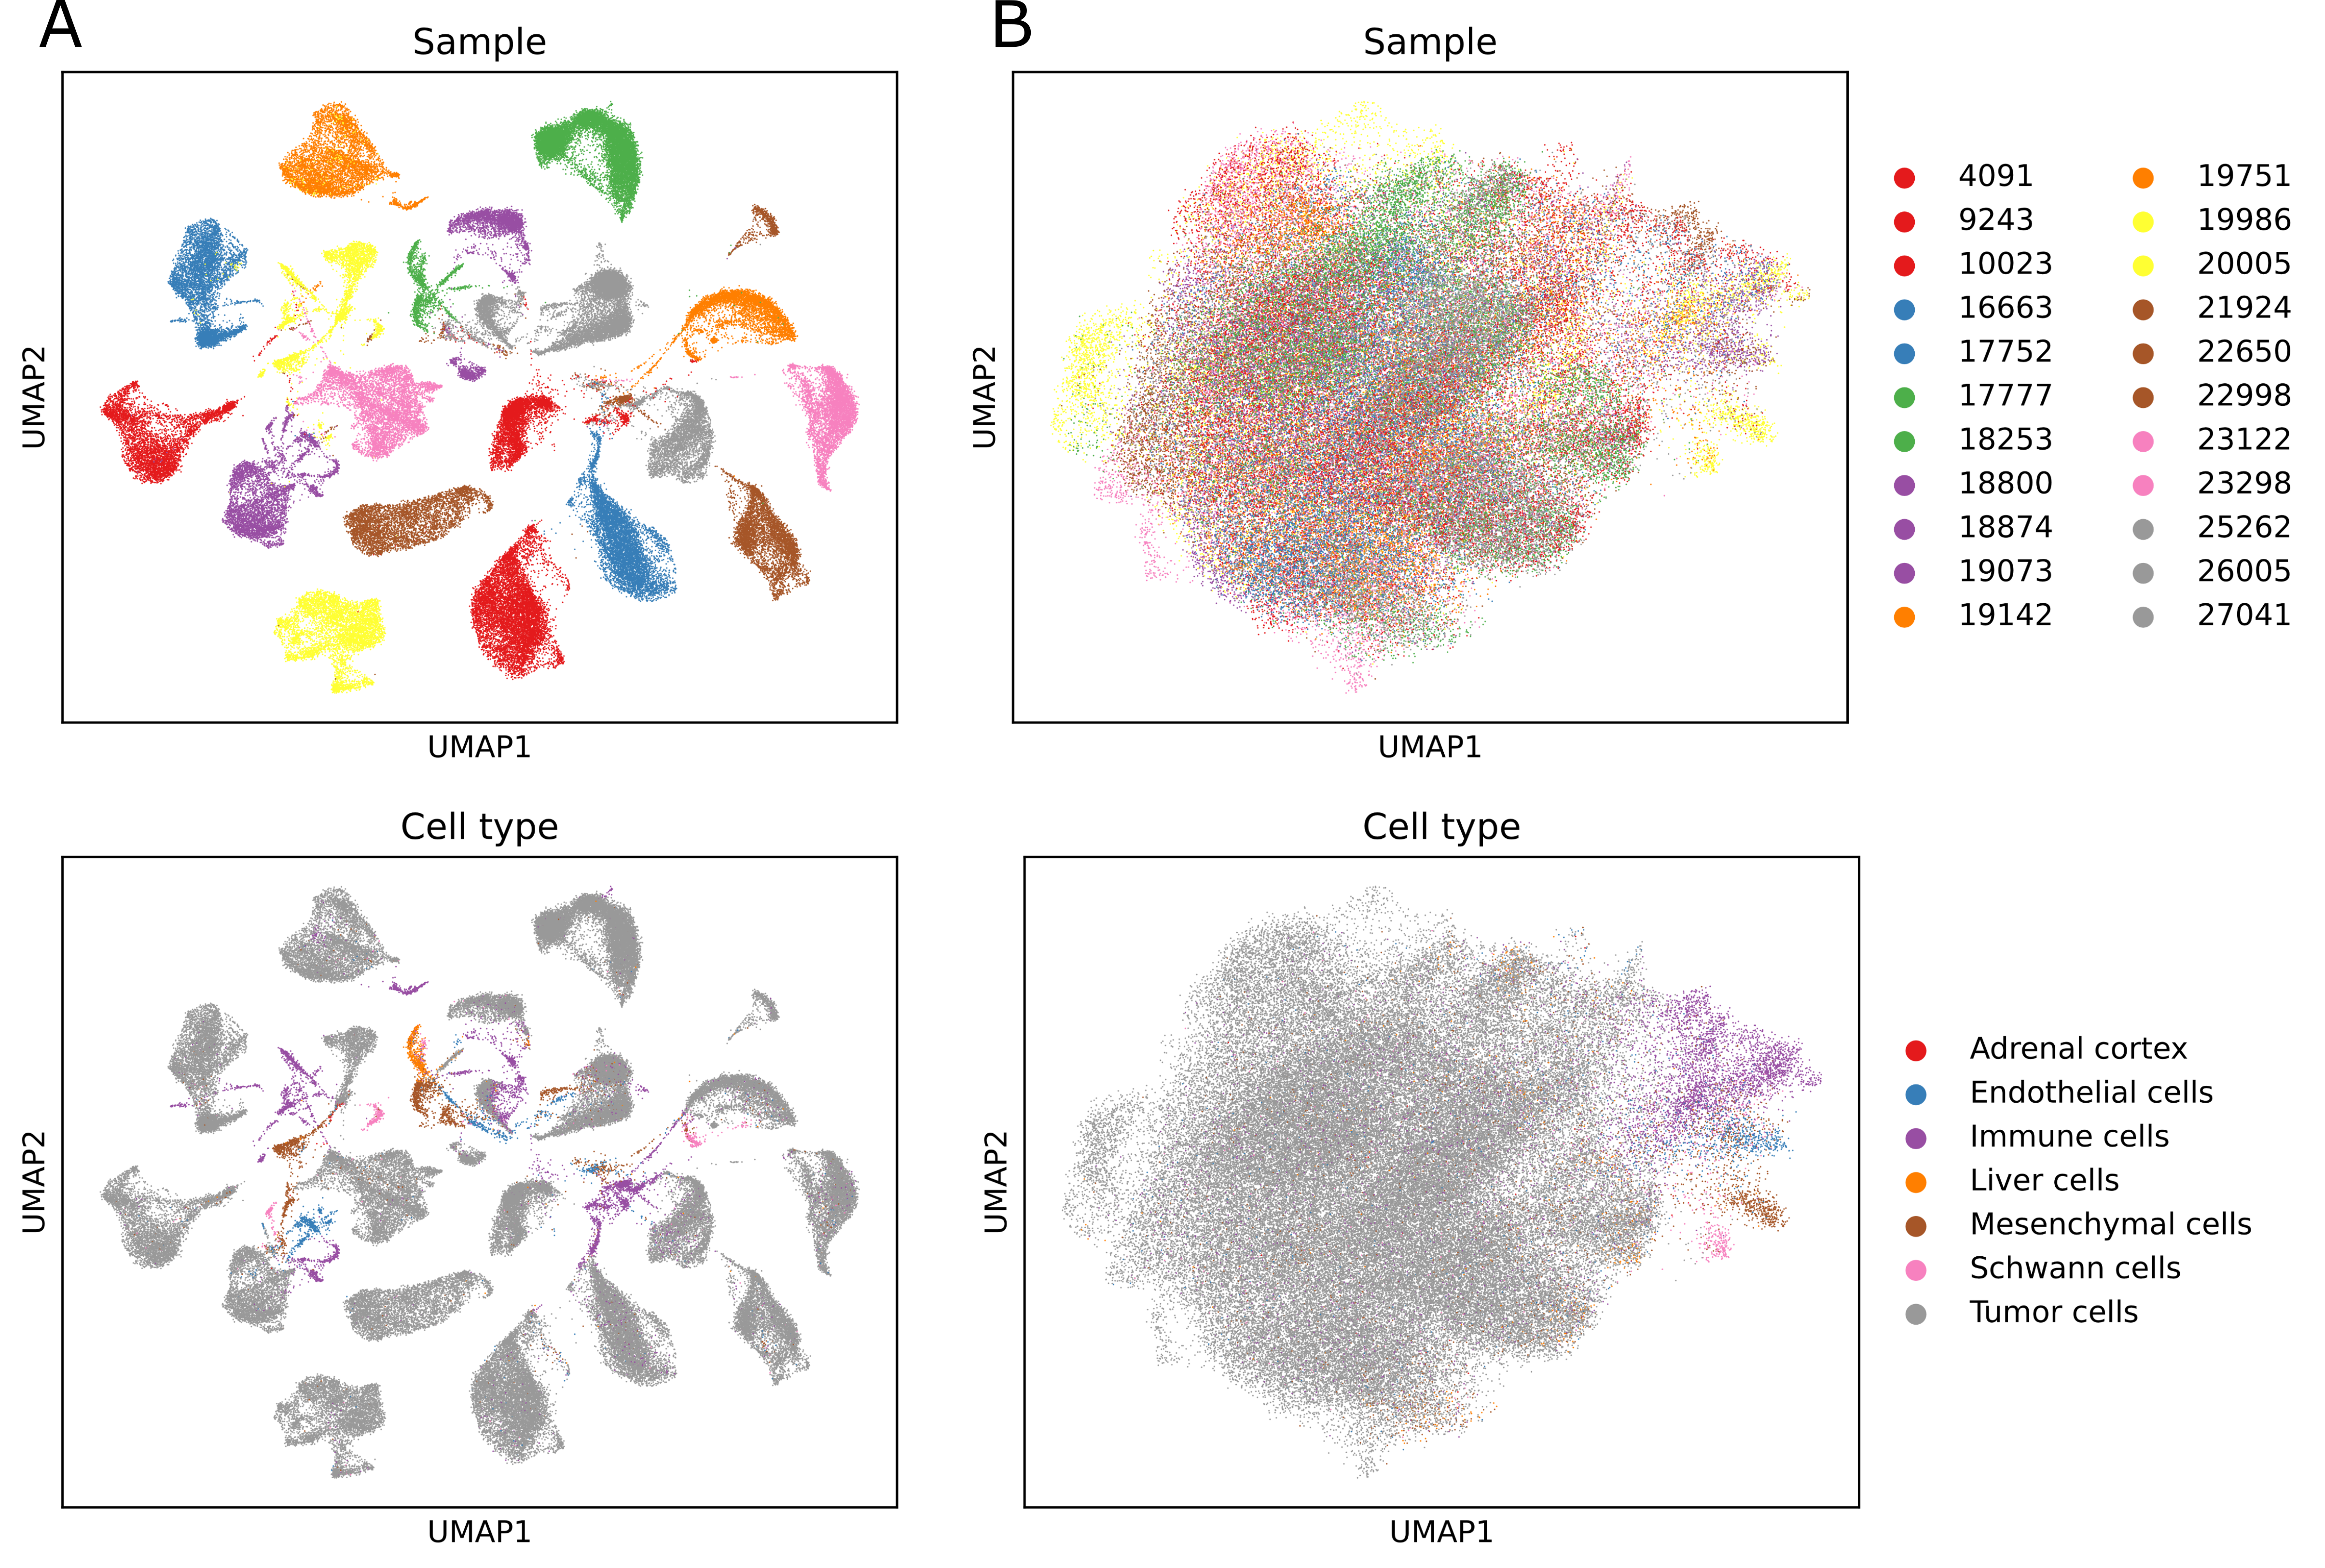
\includegraphics[scale=0.70]{SCENIC_sparse/nb_batch.png}
    \caption{\small{\textbf{Testing of batch correction function of VEGA} | We tested the function of batch correction of the model by the integration of 22 samples in the neuroblastoma dataset which suffers from severe batch effects. \textbf{(A)} The UMAP embedding of the gene expression space shows that cells were clustered mainly based on technical differences between the samples rather than biological differences between the cell types. \textbf{(B)} The UMAP embedding of the VEGA latent space shows that cells from the different samples were blended and clustered into cell types when the batch annotations were provided for the model training.}}
    \label{fig:sparse_nb_batch}
\end{figure}

\section{Model using L1 regularized linear decoder}\label{results:regularized_decoder}
In the previous work, we performed the benchmark studies on VEGA\cite{Seninge2021} and investigated some of its properties. The results demonstrated that VEGA is capable of learning biologically meaningful representations of gene expression data when correct prior knowledge was provided. However, one obvious drawback of VEGA lies in its hard-coded linear decoder. Hard-coded connections in the decoder leaves no room for further correcting or expanding existing prior biological knowledge which is usually incomplete or not context-specific\cite{Seninge2021}. To enable a model to use prior knowledge more flexibly, we employed the L1 regularization technique\cite{Ng2004} on decoder weights of unannotated relationships between GMVs and genes in the output layer, introduced in Rybakov et al. (2020). During model training,
\begin{align}
    w^{(t+1)} &= w^t - G \;\;\;\;\;\; \to \textnormal{for updating weights of annotated connections}\label{eqn:1} \\
    w^{(t+1)} &= w^t - G - \lambda\alpha|w^t| \;\;\;\;\;\; \to \textnormal{for updating weights of unannotated connections}\label{eqn:2}
\end{align}
where $w^{(t+1)}$ denotes an updated weight, $w^t$ denotes a weight before updated and $G$ represents the standard gradient descent, which describes the updating of weights of annotated relationships between GMVs and feature genes in Eq.(\ref{eqn:1}). For those weights of unannotated relationships, the weights are additionally penalized by the proximal gradient descent $\lambda\alpha|w^t|$ where $\lambda$ and $\alpha$ designate the regularization hyperparameter and the learning rate respectively, described in Eq.(\ref{eqn:2}). The product of $\lambda$ and $\alpha$ in the proximal gradient descent procedure\cite{Parikh2014} can be intuitively seen as the degree of imposing L1 regularization on weights in the decoder (see Methods \ref{methods:L1} for more details).

\subsection{Model recovers artificially removed target genes}\label{sec:L1_adm_removed}
Firstly, to gain more knowledge of how a model using the L1 regularized linear decoder works, we systematically trained a number of individual models using different values of $\lambda\alpha$ and artificially modified prior knowledge. We attempted to understand how the regularized decoder behaves when different values of $\lambda\alpha$ are employed and check whether the model is able to correct artificially modified prior knowledge. To this end, we artificially removed target genes from the aforementioned SCENIC\cite{Aibar2017} regulons inferred from the human adrenal medulla dataset\cite{Jansky2021}. For instance, we removed three target genes, \textit{EML5}, \textit{STMN2} and \textit{ALK}, from the SCENIC GATA3 regulon according to the top rankings of the GATA3 weights in the hard-coded linear decoder of VEGA (Appx.\ref{fig:L1_adm_removal_appx}A). To be clearer, the reason that we picked these three high-ranking genes of GATA3 (i.e., the weights of the connections between GATA3 and these genes are relatively high) was to first check if the model is capable of recovering the missing genes that have strong relationships with GATA3. We made a recovery plot on the GATA3 weights for each of the trained models and computed the area under the curve (AUC) to evaluate the degree of the prior used by the model (see Methods \ref{methods:recovery}). The hyperparameters used in this section can be found in Appendix \ref{appendixA}. The results show that, when $\lambda\alpha = 10^{-5}$ and $10^{-4}$, the rankings of the GATA3 annotated genes were evenly distributed over the feature list (the scaled AUC scores were both 0.51), which indicates the prior was not really used by the models (Fig.\ref{fig:L1_adm_removal}A). This finding was verified by the recovery plot on the GATA3 weights from the model using the fully connected decoder (AUC of 0.48, Appx.\ref{fig:L1_adm_removal_appx}B). From $\lambda\alpha = 10^{-3}$ to $\lambda\alpha = 0.1$, we observed the higher AUC scores, indicating that the models used the prior more evidently (Fig.\ref{fig:L1_adm_removal}A). When $\lambda\alpha = 1$, the model obtained the highest AUC score (0.91) but lost its capacity to recover the removed genes (Fig.\ref{fig:L1_adm_removal}A). Moreover, for the count of non-zero links between GATA3 and genes in the output layer (i.e., the putative GATA3 regulon), we observed that the number decreased when the model obviously started using the prior (from $\lambda\alpha = 10^{-3}$) and had a drastic drop when $\lambda\alpha$ was reaching 1 (Appx.\ref{fig:L1_adm_removal_appx}C), which is consistent with the information given by the recovery plots. Collectively, we can roughly split the behavior of the regularized decoder into three modes: The fully connected mode when $\lambda\alpha < 10^{-3}$, the regularized mode when $10^{-3} \leq \lambda\alpha < 1$ and the hard-coded mode when $\lambda\alpha = 1$. These findings hold true for all of our experiments (artificially modifying predefined gene sets), that is, the overall decoder behavior is not influenced by slightly modified prior knowledge.

Next, to investigate how the model deciphers the relationships between GATA3 and the feature list and check whether it can recover those three genes artificially removed from the SCENIC GATA3 regulon, we ranked the genes in order of their tuned weights. The results show that, when $\lambda\alpha = 10^{-5}$ and $10^{-4}$, the top 20 high-ranking genes of GATA3 were mostly not in the SCENIC GATA3 regulon (Fig.\ref{fig:L1_adm_removal}B), and from $\lambda\alpha = 10^{-3}$ to $\lambda\alpha = 1$, the top 20 high-ranking genes were gradually filled with GATA3 target genes (Fig.\ref{fig:L1_adm_removal}B), which corroborates our earlier conclusion of the model behavior in terms of different $\lambda\alpha$ values used. Furthermore, when looking into the rankings of those three removed genes, we found the model using $\lambda\alpha = 10^{-3}$ could best recover the removed genes and the models using the other $\lambda\alpha$ values diverging from $\lambda\alpha = 10^{-3}$ (either to the fully connected mode or to the hard-coded mode) had worse recovering performance (Table \ref{table:L1_removal_ranking}). This result made those genes which were high-ranking but not from the SCENIC GATA3 regulon in the model using $\lambda\alpha = 10^{-3}$ extremely intriguing. After checking research papers and existing databases, we found, for example, \textit{LINGO2} and \textit{CTNND2} are significantly upregulated in CD4+ T cells when GATA3 is knocked down by siRNA\cite{Feng2020} and \textit{AGBL4} is bound by GATA3 according to TF binding site profiles measured by ChIP-seq from the ENCODE Project\cite{ENCODE2004,ENCODE2011,Rouillard2016}. These pieces of biological evidence indicates the inferred target genes are associated with GATA3, yet, they are not in the context of adrenal medullary cells. Consequently, further work on verifying whether those inferred genes are truly regulated by GATA3 in adrenal medullary cells is needed. Together, the model using $\lambda\alpha = 10^{-3}$ can best recover the missing genes artificially removed from the prior and potentially infer some other possible target genes.

Apart from GATA3, we performed the same analyses on another TF, JUN, to double check if the behavior of the regularized linear decoder is as our earlier findings. We artificially removed three target genes, \textit{DDC}, \textit{ROBO1} and \textit{GRK5}, from the SCENIC JUN regulon in the same manner as described above. We observed the very similar model behavior that the decoder behaved in a more fully connected way when $\lambda\alpha < 10^{-3}$, in a regularized way when $10^{-3} \leq \lambda\alpha < 1$ and in a hard-coded way when $\lambda\alpha = 1$ (Appx.\ref{fig:L1_adm_removal_appx}D,E). Interestingly, the model also best recovered the removed genes when $\lambda\alpha = 10^{-3}$, which is in line with the experiment on GATA3 (Table \ref{table:L1_removal_ranking}). For those genes which were high-ranking but not from the SCENIC JUN regulon in the model using $\lambda\alpha = 10^{-3}$ (Appx.\ref{fig:L1_adm_removal_appx}E), we found that \textit{SLC7A5} and \textit{HSP90AA1} are both bound by JUN according to the previous studies\cite{ENCODE2004,ENCODE2011,Rouillard2016,Lachmann2010} and \textit{SLC7A5} is significantly upregulated in BT-549 cells from the mammary gland when JUN is knocked down by siRNA\cite{Feng2020}. Again, since the evidence supporting the relationships between JUN and inferred target genes is not context-specific, further work on confirming the inferences is needed. In conclusion, the model using the L1 regularized linear decoder can successfully recover the artificially removed target genes and potentially expand the existing TF target gene sets.\vspace{3cm}

\begin{figure}[b!]
    \caption{\small{\textbf{Investigation of regularized decoder behavior} | We artificially removed three genes from the SCENIC regulons inferred from the human adrenal medulla data to investigate the general behavior and the ability to recover the missing target genes of the regularized decoder. Collectively, the results show that the decoder behaved in a fully connected way when $\lambda\alpha < 10^{-3}$, in a regularized way when $10^{-3} \leq \lambda\alpha < 1$ and in a hard-coded way when $\lambda\alpha = 1$. \textbf{(A)} The x-axis indicates the ranking of the weights of a certain GMV (i.e.,GATA3) to the gene reconstructions in the decoder and if the corresponding gene was annotated in the SCENIC GATA3 regulon, the frequency increased 1 in the y-axis. The recovery plots display the increasing AUC scores when the values of $\lambda\alpha$ increased. The red bar on a curve indicates the number of non-zero weights of GATA3 (i.e., the putative GATA3 regulon). Note that the zero-valued weights were randomly ranked. \textbf{(B)} The x-axis indicates the top 20 high-ranking genes (highest weights) of GATA3 and the y-axis indicates the weight magnitude. The plots show that most of the high-ranking genes were not annotated in the SCENIC GATA3 regulon (colored in black) when $\lambda\alpha < 10^{-3}$ and with increasing $\lambda\alpha$ vlues, the top 20 high-ranking genes were gradually filled with genes annotated in the SCENIC GATA3 regulon (colored in red). Gene names prefixed by double asterisks indicate the artificially removed genes.}}
\end{figure}

\addtocounter{figure}{-1}
\begin{figure}[H]
    \centering
    \vspace{2.4cm}
    \includegraphics[scale=0.72]{SCENIC_L1/adm_L1_removal.png}
    \caption{\small{The caption is on the previous page.}}
    \label{fig:L1_adm_removal}
\end{figure}

\newpage

\begin{table}[h!]
    \begin{center}
        \captionsetup{width=.76\textwidth}
        \caption{\small{\textbf{Rankings of artificially removed genes} | \textit{EML5}, \textit{STMN2} and \textit{ALK} were artificially removed from the SCENIC GATA3 regulon and \textit{DDC}, \textit{ROBO1} and \textit{GRK5} were artificially removed from the SCENIC JUN regulon. NA indicates that the weight of GATA3 or JUN to the certain gene reconstruction was zero, which means the artificially removed gene was not recovered.}}
        \label{table:L1_removal_ranking}
        \begin{tabular}{|c|c|c|c|c|c|c|}
        \hline
        & \small{GATA3} & & & \small{JUN} & &\\
        & \small{\textit{\textbf{EML5}}} & \small{\textit{\textbf{STMN2}}} & \small{\textit{\textbf{ALK}}} & \small{\textit{\textbf{DDC}}} & \small{\textit{\textbf{ROBO1}}} & \small{\textit{\textbf{GRK5}}}\\
        \hline
        \small{\boldmath{$\lambda\alpha = 10^{-5}$}} & \small{838} & \small{NA} & \small{110} & \small{22} & \small{773} & \small{6}\\
        \hline
        \small{\boldmath{$\lambda\alpha = 10^{-4}$}} & \small{1430} & \small{NA} & \small{121} & \small{293} & \small{NA} & \small{138}\\
        \hline
        \small{\boldmath{$\lambda\alpha = 10^{-3}$}} & \textbf{7} & \textbf{29} & \textbf{32} & \textbf{114} & \textbf{102} & \textbf{105}\\
        \hline
        \small{\boldmath{$\lambda\alpha = 10^{-2}$}} & \small{77} & \small{55} & \small{59} & \small{118} & \small{738} & \small{126}\\
        \hline
        \small{\boldmath{$\lambda\alpha = 0.1$}} & \small{81} & \small{64} & \small{80} & \small{155} & \small{NA} & \small{169}\\
        \hline
        \small{\boldmath{$\lambda\alpha = 1$}} & \small{NA} & \small{NA} & \small{NA} & \small{NA} & \small{NA} & \small{NA}\\
        \hline
        \end{tabular}
    \end{center}
\end{table}

\subsection{Model excludes artificially added genes}\label{sec:L1_adm_added}
Secondly, we investigated how the model using the L1 regularized decoder treats artificially added genes in prior knowledge using the same human adrenal medulla dataset\cite{Jansky2021} and the same strategy described in Section \ref{sec:L1_adm_removed}. Since we observed that the regularized decoder tends to capture genes whose expression levels are averagely high for regulon inferences, i.e., a large proportion of high-ranking putative target genes of a TF have high average expression levels in the single-cell transcriptome data, e.g., GATA3 (Fig.\ref{fig:L1_adm_removal}B), we were inspired to study the behavior of the regularized decoder in two aspects: Artificially adding genes with either high average expression levels or low average expression levels. The way we selected added genes was computing the mean of expression values of each gene across all cells, ranking the genes based on the average expression levels and avoiding picked genes being biologically meaningful to a certain regulon by looked over a couple of existing databases, such as DoRothEA\cite{Garcia-Alonso2019}, Harmonizome\cite{Rouillard2016}, KnockTF\cite{Feng2020}, etc. For instance, we artificially added three genes with high expression levels: \textit{GNAS}, \textit{MEG8} and \textit{NRXN1} and three genes with low expression levels: \textit{PRDM16}, \textit{MEGF6} and \textit{AJAP1} into the SCENIC GATA3 regulons in the duplicate files containing the prior to create two versions of modified prior knowledge. We then systematically trained several individual models using different $\lambda\alpha$ values and these two versions of artificially modified prior knowledge and checked the rankings of weights of the artificially added non-biologically meaningful genes. The hyperparameters used in this task can be found in Appendix \ref{appendixA}. Notice that the behavior of the regularized decoder using different $\lambda\alpha$ values is very similar to our previous findings that the regularized decoder behaves in a more fully-connected way when $\lambda\alpha < 10^{-3}$, in a regularized way when $10^{-3} \leq \lambda\alpha < 1$ and in a hard-coded way when $\lambda\alpha = 1$ (Appx.\ref{fig:L1_adm_addition_appx}). The results show that, when $\lambda\alpha = 10^{-5}$ and $10^{-4}$, the artificially added genes with high expression levels had the higher average rankings than the added genes with low expression levels, which is in line with our previous observations that the decoder tends to capture genes with high average expression levels (Table \ref{table:L1_addition_ranking_GATA3}). Theoretically, the reason might be that genes with high average expression levels usually indicates that genes also have high variances, which might need larger weights to take care of more variable gene reconstructions in the decoder. When $10^{-3} \leq \lambda\alpha < 1$ where the regularized decoder uses the prior evidently, some of the artificially added genes could be excluded, yet the changes in the rankings across different $\lambda\alpha$ values did not have a clear pattern (Table \ref{table:L1_addition_ranking_GATA3}). Roughly, the regularized decoder could best exclude the artificially added genes with high and low expression levels when $\lambda\alpha = 0.1$. Interestingly, when $\lambda\alpha = 1$, all of the artificially added genes with low expression levels were excluded while the added genes with high expression levels were kept, which corroborates again that genes with high expression levels (high variances) are more likely to be captured by the decoder (Table \ref{table:L1_addition_ranking_GATA3}).

Similarly, apart from GATA3, we performed the same analyses on another TF, JUN. We artificially added three genes with high expression levels: \textit{RBFOX1}, \textit{MEG8} and \textit{DLGAP1} and three genes with low expression levels: \textit{PRDM16}, \textit{TSHR} and \textit{PTPRT} into the SCENIC JUN regulons in the duplicate files containing the prior information. At first glance, the ranking results of these added genes from JUN are not very similar to those from GATA3. When $\lambda\alpha = 10^{-5}$ and $10^{-4}$, there was no obvious contrast between the rankings of the artificially added genes with high expression levels and those with low expression levels and, interestingly, \textit{RBFOX1} whose expression level is averagely high was not captured by the decoder, which is not in line with our earlier hypothesis and finding in the example of GATA3 (Table \ref{table:L1_addition_ranking_JUN}). When $10^{-3} \leq \lambda\alpha < 1$, in general, the artificially added genes acquired higher rankings when $\lambda\alpha$ increased and the regularized decoder seemed to be able to exclude the added genes with low expression levels when $\lambda\alpha$ was set to $10^{-2}$ (Table \ref{table:L1_addition_ranking_JUN}). When $\lambda\alpha = 1$, all of the artificially added genes were kept except \textit{PRDM16} and the added genes with high expression levels had the higher average ranking than those with low expression levels (Table \ref{table:L1_addition_ranking_JUN}). Collectively, the regularized decoder has the potential to exclude artificially added non-biologically meaningful genes, yet there is no specific pattern on how the regularized decoder behaves with different values of $\lambda\alpha$. Therefore, further work on how to generalize this technique to all genes is needed.

\begin{table}[h!]
    \begin{center}
        \captionsetup{width=.83\textwidth}
        \caption{\small{\textbf{Rankings of artificially added genes in SCENIC GATA3 regulon} | We split the task into two parts: artificially adding the genes with high average expression levels (\textit{GNAS}, \textit{MEG8} and \textit{NRXN1}) and the genes with low average expression levels (\textit{PRDM16}, \textit{MEGF6} and \textit{AJAP1}) into the SCENIC GATA3 regulons in the duplicate files containing the prior. The rankings marked in bold represent relatively better outcomes of our testing. NA indicates that the weight of GATA3 to the certain gene reconstruction was zero, which means the artificially added gene was not included in the putative GATA3 regulon.}}
        \label{table:L1_addition_ranking_GATA3}
        \begin{tabular}{|c|c|c|c|c|c|c|}
        \hline
        & \small{HIGH} & & & \small{LOW} & &\\
        & \small{\textit{\textbf{GNAS}}} & \small{\textit{\textbf{MEG8}}} & \small{\textit{\textbf{NRXN1}}} & \small{\textit{\textbf{PRDM16}}} & \small{\textit{\textbf{MEGF6}}} & \small{\textit{\textbf{AJAP1}}}\\
        \hline
        \small{\boldmath{$\lambda\alpha = 10^{-5}$}} & \small{17} & \small{12} & \small{724} & \small{1158} & \small{NA} & \small{196}\\
        \hline
        \small{\boldmath{$\lambda\alpha = 10^{-4}$}} & \small{21} & \small{2} & \small{503} & \small{1024} & \small{303} & \small{NA}\\
        \hline
        \small{\boldmath{$\lambda\alpha = 10^{-3}$}} & \small{71} & \small{NA} & \small{242} & \small{NA} & \small{348} & \small{440}\\
        \hline
        \small{\boldmath{$\lambda\alpha = 10^{-2}$}} & \small{936} & \small{NA} & \small{NA} & \small{NA} & \small{143} & \small{191}\\
        \hline
        \small{\boldmath{$\lambda\alpha = 0.1$}} & \textbf{603} & \textbf{NA} & \textbf{NA} & \textbf{951} & \textbf{NA} & \textbf{166}\\
        \hline
        \small{\boldmath{$\lambda\alpha = 1$}} & \small{35} & \small{14} & \small{94} & \small{NA} & \small{NA} & \small{NA}\\
        \hline
        \end{tabular}
    \end{center}
\end{table}

\begin{table}[h!]
    \begin{center}
        \captionsetup{width=.86\textwidth}
        \caption{\small{\textbf{Rankings of artificially added genes in SCENIC JUN regulon} | We split the task into two parts: artificially adding the genes with high average expression levels (\textit{RBFOX1}, \textit{MEG8} and \textit{DLGAP1}) and the genes with low average expression levels (\textit{PRDM16}, \textit{TSHR} and \textit{PTPRT}) into the SCENIC JUN regulons in the duplicate files containing the prior. The rankings marked in bold represent relatively better outcomes of our testing. NA indicates that the weight of JUN to the certain gene reconstruction was zero, which means the artificially added gene was not included in the putative JUN regulon.}}
        \label{table:L1_addition_ranking_JUN}
        \begin{tabular}{|c|c|c|c|c|c|c|}
        \hline
        & \small{HIGH} & & & \small{LOW} & &\\
        & \small{\textit{\textbf{RBFOX1}}} & \small{\textit{\textbf{MEG8}}} & \small{\textit{\textbf{DLGAP1}}} & \small{\textit{\textbf{PRDM16}}} & \small{\textit{\textbf{TSHR}}} & \small{\textit{\textbf{PTPRT}}}\\
        \hline
        \small{\boldmath{$\lambda\alpha = 10^{-5}$}} & \small{NA} & \small{325} & \small{893} & \small{628} & \small{794} & \small{NA}\\
        \hline
        \small{\boldmath{$\lambda\alpha = 10^{-4}$}} & \small{NA} & \small{663} & \small{590} & \small{708} & \small{1038} & \small{1000}\\
        \hline
        \small{\boldmath{$\lambda\alpha = 10^{-3}$}} & \small{894} & \small{51} & \small{NA} & \small{967} & \small{385} & \small{NA}\\
        \hline
        \small{\boldmath{$\lambda\alpha = 10^{-2}$}} & \small{13} & \small{17} & \small{201} & \textbf{NA} & \textbf{NA} & \textbf{379}\\
        \hline
        \small{\boldmath{$\lambda\alpha = 0.1$}} & \small{4} & \small{8} & \small{110} & \small{544} & \small{114} & \small{115}\\
        \hline
        \small{\boldmath{$\lambda\alpha = 1$}} & \small{6} & \small{1} & \small{53} & \small{NA} & \small{172} & \small{169}\\
        \hline
        \end{tabular}
    \end{center}
\end{table}

\subsection{Model infers dataset-specific GRNs using general regulons as prior}\label{sec:L1_dorothea}
In a real-world scenario, existing resources where we require prior biological knowledge are usually not context-specific, but some of those unannotated genes might play an important role in certain biological processes in certain tissues or cells\cite{Seninge2021}. In the previous tasks, we systematically studied the behavior of the model using the regularized linear decoder when the provided SCENIC regulons were artificially modified. We observed that the model was able to recover the artificially removed target genes and exclude the artificially added non-biologically meaningful genes with certain $\lambda\alpha$ values. We further asked whether the model can infer dataset-specific GRNs in the decoder using general regulons as prior knowledge and provide the biologically meaningful latent space. Similarly to the previous strategy and sticking to the human adrenal medulla dataset\cite{Jansky2021}, we systematically trained several individual models using different $\lambda\alpha$ values and the aforementioned DoRothEA\cite{Garcia-Alonso2019} regulons as the prior. The hyperparameters used in this task can be found in Appendix \ref{appendixA}. Since the decoder behaves in a more fully-connected way when $\lambda\alpha < 10^{-3}$ according to our previous observation, we focused on the values of $\lambda\alpha$ between $10^{-3}$ and 1, which makes the decoder in the regularized and hard-coded modes (Fig.\ref{fig:L1_adm_removal}A). The reason that we included the model whose decoder has no freedom to make further inferences about dataset-specific GRNs (when $\lambda\alpha = 1$) was to provide the control group, the contrast to the regularized decoder. We evaluated the inference capacity of the regularized decoder by making recovery plots on the weights of six TFs of interest (GATA3, ETS1, TFAP2B, JUN, FOS and SOX11) based on the corresponding SCENIC regulons and computing the AUC scores of them (see Methods \ref{methods:recovery}). The regularized decoder is considered having the better inference capacity when the AUC scores of those recovery plots are higher, which indicates the greater number of the high-ranking putative target genes are annotated in the SCENIC regulons. Besides, since the DoRothEA and the SCENIC regulons barely overlap with each other (Table \ref{table:dorothea_scenic_outline}), we also included the recovery curves based on the DoRothEA regulons to investigate how the regularized decoder treats those target genes from the DoRothEA prior. The results show that, in general, the inference performance of the regularized decoder was gradually ameliorated when the values of $\lambda\alpha$ increased (increasing AUC scores), except the inference of the GATA3 regulon, and had the best inference capacity when $\lambda\alpha = 0.9$ (Fig.\ref{fig:L1_adm_dorothea_hvgA}A, blue curves). As expected, when $\lambda\alpha = 1$, the regularized decoder lost its inference capacity because of a hard-coded nature of the decoder (Fig.\ref{fig:L1_adm_dorothea_hvgA}A, blue curves). For the gene regulatory information provided by the DoRothEA regulons, as the regular behavior of the regularized decoder, the prior was used more evidently when the $\lambda\alpha$ values increased, which indicates the model preserved the target genes from the DoRothEA regulons while making the inferences about the SCENIC regulons (Fig.\ref{fig:L1_adm_dorothea_hvgA}A, green curves). Furthermore, to check the interpretability in the latent space, we performed UMAP and differential activity analysis on the embedding of the model using $\lambda\alpha = 0.9$, which had the best inference performance. The UMAP plot shows that the model could well cluster cells into cell types and preserve the developmental trajectories of the adrenal medulla (Fig.\ref{fig:L1_adm_dorothea_hvgBC}B). The volcano plots reveal that the model could capture more cell type-specific differential TF activities compared to the results from VEGA using the DoRothEA regulons as the prior (Fig.\ref{fig:sparse_adm_dorothea_hvg}B), yet some of those significantly differential TF activities were falsely predicted, e.g., CUX1, NFATC1 and NR2F2 (Fig.\ref{fig:L1_adm_dorothea_hvgBC}C). Note that the differential activity analysis results took Fig.\ref{fig:sparse_adm_scenic}C as references. Together, the model has the potential to infer dataset-specific GRNs in the regularized decoder using general regulons as prior knowledge and provide the interpretable context-specific latent space.

Next, to verify the more data-specific regulons inferred by the model were truly based on the DoRothEA regulons, we randomized the DoRothEA gene sets to different degrees (10\%, 50\% and 90\%) to investigate whether the regularized decoder can still keep the inference capacity (see Methods \ref{methods:randomization}). We expected that the regularized decoder should lose its inference capacity when the DoRothEA gene sets are greatly randomized, which indicates the reasonable general regulons as the prior are critical for making inferences about more specific GRNs. Similarly to the description above, the recovery curves based on the SCENIC and the DoRothEA regulons were both included, but we will mainly focus on the observations of the changes in the inference performance of the regularized decoder (blue curves). We first looked into the model with $\lambda\alpha = 0.9$, which had the best inference performance. We observed that, when 10\% and 50\% of the DoRothEA target genes were shuffled, the changes in the inference performance (AUC scores) did not have a clear pattern (Fig.\ref{fig:L1_adm_dorothea_hvgD}D). In some cases, the regularized decoder had the better inference performance when using the randomized DoRothEA gene sets than using the original ones, e.g., GATA3 and in other cases, the better inferences happened when using the 50\% randomized DoRothEA gene sets compared to using the 30\% randomized ones, e.g., TFAP2B. The reason for these results may be that, owing to the low degree of overlapping between the DoRothEA and the SCENIC regulons, some unannotated genes which play an important role in the GRN reconstructions were put into corresponding regulons and some unimportant target genes were removed from regulons during the randomization procedure. Even so, when the DoRothEA target genes were 90\% randomized, nearly all of the GRN inferences, except GATA3, had the low AUC scores which are very similar to the scores obtained from the regularized decoder using the original DoRothEA regulons as prior knowledge when $\lambda\alpha = 1$ (Fig.\ref{fig:L1_adm_dorothea_hvgA}A), which indicates the decoder could not faithfully infer the SCENIC regulons (Fig.\ref{fig:L1_adm_dorothea_hvgD}D). Considering that using $\lambda\alpha = 0.9$ did not give the regularized decoder much freedom to make the inferences, we also looked into the model with $\lambda\alpha = 0.5$ as the sanity check, which had the poorer inference performance than the model with $\lambda\alpha = 0.9$ but still had a tendency to infer the SCENIC regulons. Similarly to the model with $\lambda\alpha = 0.9$, when 10\% and 50\% of the DoRothEA target genes were randomized, the changes in the inference performance did not have an obvious pattern, but when the DoRothEA target genes were 90\% randomized, most of the GRN inferences, except GATA3 and TFAP2B, were lost (Appx.\ref{fig:L1_adm_dorothea_rand_0.5_hvg}). Together, using the reasonable general regulons as prior knowledge is important for the model to make further inferences about more data-specific GRNs in the decoder.

\begin{figure}[b!]
    \caption{\small{\textbf{Context-specific GRN inferences from general prior GRNs} | We trained the model with the regularized decoder on the human adrenal medulla dataset and using the non-context-specific DoRothEA regulons as prior knowledge in an attempt to infer more dataset-specific GRNs. \textbf{(A)} The x-axis indicates the ranking of weights of a certain TF and if the corresponding gene was annotated in the SCENIC regulon (blue curves) or in the DoRothEA regulon (green curves) of the TF, the frequency increased 1 in the y-axis. Note that we will focus on blue curves for investigating the changes in the inference performance of the regularized decoder across different $\lambda\alpha$ values. The columns and the rows of the panel A show the different values of $\lambda\alpha$ and the different TFs. The recovery plots show that the regularized decoder had the best inference performance when $\lambda\alpha = 0.9$ and lost its inference capacity when $\lambda\alpha = 1$ (equivalent to the hard-coded decoder). The red bar on a curve indicates the number of non-zero weights of a certain TF (i.e., the putative regulon of the TF). Note that the zero-valued weights were randomly ranked. \textbf{(B)} The UMAP embedding of the latent space from the model with $\lambda\alpha = 0.9$ shows the clear cell clustering and the developmental trajectories of the adrenal medulla. \textbf{(C)} The x-axis and the y-axis indicate the significance level and the mean absolute difference of GMV activity comparisons between two cell types. The volcano plots reveal that the model using the regularized decoder with $\lambda\alpha = 0.9$ could capture more cell type-specific differential TF activities than using the hard-coded decoder (Fig.\ref{fig:sparse_adm_dorothea_hvg}B), yet there were also slightly more wrongly predicted significantly differential TF activities (colored in green). We considered TFs to be significantly differentially activated when $|\textnormal{log}_e(\textnormal{BF})|>3$. \textbf{(D)} To verify the more dataset-specific regulons were truly inferred from the DoRothEA regulons, we trained the model with $\lambda\alpha = 0.9$ using the prior which was randomized to different levels to investigate the changes in the performance of decoder inferences. The columns and the rows of the panel D show the different TFs and the different degrees of randomization of the prior. The results show that there was no evident pattern of the changes in the inference performance when the prior was 10\% and 50\% randomized and nearly all of the GRN inferences, except GATA3, were lost when the prior was 90\% randomized. Ori indicates the original prior and Rand indicates the degree of randomization of the prior.}}
\end{figure}

\addtocounter{figure}{-1}
\begin{figure}[h!]
    \centering
    \hspace*{-1mm}
    \includegraphics[scale=0.7]{DoRothEA_L1/adm_dorothea_L1_hvg.png}
    \caption{\small{The caption is on the previous page.}}
    \label{fig:L1_adm_dorothea_hvgA}
\end{figure}

\addtocounter{figure}{-1}
\begin{figure}[h!]
    \centering
    \hspace*{-4mm}
    \includegraphics[scale=0.76]{DoRothEA_L1/adm_dorothea_L1_hvg2.png}
    \caption{\small{This figure is continued from the previous page.}}
    \label{fig:L1_adm_dorothea_hvgBC}
\end{figure}

\addtocounter{figure}{-1}
\begin{figure}[h!]
    \centering
    \hspace*{-5mm}
    \includegraphics[scale=0.69]{DoRothEA_L1/adm_dorothea_L1_hvg3.png}
    \caption{\small{This figure is continued from the previous page.}}
    \label{fig:L1_adm_dorothea_hvgD}
\end{figure}


\chapter{Discussion}
In this work, we investigated the ability and various properties of two kinds of interpretable VAEs which are used to analyze single-cell transcriptomes, introduced in Seninge et al. (2021) and Rybakov et al. (2020) respectively. Firstly, VEGA\cite{Seninge2021} hard codes the wiring of its single-layer linear decoder through a binary mask that is subject to prior biological knowledge. By limiting the connection of latent variables to certain sets of genes in the output layer, the latent variables can be modeled as a list of gene modules depending on provided prior knowledge. This operation makes VEGA extremely flexible to take advantage of diverse sorts of known biology as prior knowledge, such as pathways, GRNs and cell type marker genes, as long as the prior consists of biologically meaningful gene sets, which enables us to interpret single-cell transcriptomes from many other different viewpoints. From another perspective, VEGA provides an efficient way of inferring the activity of gene modules from transcriptomic data at the single-cell level. To be more concrete, in our work, we analyzed the human adrenal medulla dataset\cite{Jansky2021} using the SCENIC regulons\cite{Jansky2021} inferred from the same dataset as the prior to infer the TF activities of individual adrenal medullary cells. Note that VEGA can be seen as an alternative method to the AUCell algorithm in the SCENIC workflow\cite{Aibar2017}, which aims at scoring \textit{a priori} gene sets to identify active TF activities in every single cell. Next, the interpretable VEGA embedding containing inferred gene module activities of all cells can be used for many downstream studies, such as cell type identities, cellular states of different cell populations and so on. Since each GMV is encoded into the posterior distribution, it also provides a natural way of conducting various types of hypothesis testing, e.g., GMV differential activity analysis\cite{Seninge2021} used in this work. Our analysis results demonstrate the potential of VEGA in terms of inferring reasonable GMV activities from single-cell transcriptomic data when prior knowledge is provided to guide the decoder wiring (see Section \ref{sec:sparse_adm} in Results). Apart from the TFs of interest based on the inferred TF activity result obtained using the AUCell algorithm (Fig.\ref{fig:sparse_adm_scenic}C), VEGA also captured some other significantly differential TF activities between different cell types (Appx.\ref{fig:sparse_adm_scenic_appx}D), which is worth further investigation. However, we did not find any supporting biological evidence for them from previous studies. Therefore, whether these significantly differential TF activities are biologically meaningful or false positives remains unclear.

For the model reproducibility which is important to the core value of VEGA, interpretability, we observed that using a dropout layer in the latent space improves the overall model training stability (see Section \ref{sec:reproducibility} in Results). Besides, using a dropout layer in the latent space also has been proved to be an effective way of preserving the redundancy between similar GMVs (i.e., prior gene modules whose gene sets are overlapped with each other)\cite{Seninge2021}. However, there were still a number of unrelated or even anticorrelated GMVs between two individual trained models, and we found that a subgroup of GMVs whose decoder wiring is highly similar tend to have low correlations. Note that the PBMCs dataset\cite{Kang2018} and the Reactome pathways\cite{Jassal2020} are discussed in this part. For example, we observed that the GMVs representing the Notch signaling pathways (NOTCH2, NOTCH3 and NOTCH4) whose gene sets are 92\% overlapped with each other had the poor reproducibility despite a dropout layer used in the latent space (Table \ref{table:notch}). The reason may be that the learned GMV-specific information is randomly distributed over these highly similar GMVs due to the overlapping decoder connections, so the information these GMVs hold will be more variable from training to training, which also implies the loss of the GMV interpretability. Yet, highly overlapping prior gene sets is not always the cause because we also observed subgroups of highly similar GMVs had the favorable reproducibility. Therefore, further work on discerning causes of poor reproducibility and finding a way to adress this issue for generalizing the model to possibly all gene modules is needed.

\begin{table}[h!]
    \begin{center}
        \captionsetup{width=.73\textwidth}
        \caption{\small{\textbf{Example of poor reproducibility of highly overlapping gene modules} | $z\_dropout$ indicates the dropout rate of a dropout layer used in the latent space. The numeric values indicate the PCC of a certain gene module between two individual trained models.}}
        \label{table:notch}
        \begin{tabular}{|c|c|c|c|}
        \hline
        & \textbf{\small{\boldmath{$z\_dropout=0$}}} & \textbf{\small{\boldmath{$z\_dropout=0.3$}}} & \textbf{\small{\boldmath{$z\_dropout=0.5$}}}\\
        \hline
        \textbf{\small{NOTCH2}} & \small{0.006} & \small{0.308} & \small{0.238}\\
        \hline
        \textbf{\small{NOTCH3}} & \small{0.013} & \small{0.320} & \small{0.189}\\
        \hline
        \textbf{\small{NOTCH4}} & \small{0.018} & \small{0.333} & \small{0.219}\\
        \hline
        \end{tabular}
    \end{center}
\end{table}

Secondly, one big limitation of VEGA lies in its hard-coded decoder which leaves no room for further correcting or expanding existing biological knowledge bases\cite{Seninge2021}. To this end, instead of hard coding, the L1 regularization technique can be selectively employed on weights in the single-layer linear decoder through a binary mask based on the prior. By penalizing the weight of decoder connections that are not included in the prior (i.e., gradually shrinking the weight of unannotated relationships between GMVs and genes to zero), the model has a chance to preserve potentially important unannotated genes for a certain gene module and in the meantime, can exclude computationally unassociated genes. Note that the human adrenal medulla dataset\cite{Jansky2021} and the SCENIC adrenal medulla regulons\cite{Jansky2021} are discussed in this part. Our experimental results indicate that the model using the regularized decoder had the ability to recover the missing target genes and expand the SCENIC adrenal medulla regulons (see Section \ref{sec:L1_adm_removed} in Results). However, for non-biologically meaningful genes, the model could exclude them in certain conditions but there was no clear pattern of how the regularized decoder handle those artificially added genes (see Section \ref{sec:L1_adm_added} in Results). Besides, we observed that genes with a high average expression level are more likely to have high weight values. Theoretically, the reason might be that genes having a high expression level usually indicate they also have high variance, so they need higher weights to take care of the reconstruction of more variable gene expression levels. Generally, we regard the weight of decoder connections as the strength of relationships between GMVs and genes, yet whether the decoder weights are biologically meaningful or just computationally meaningful needs further investigation.

Moreover, we used the non-context-specific DoRothEA regulons\cite{Garcia-Alonso2019} as the prior in an attempt to infer more dataset-specific regulons (see Section \ref{sec:L1_dorothea}). Our experimental results show that the model using the regularized decoder can potentially infer more dataset-specific GRNs from the DoRothEA regulons. However, we also observed that the inference of dataset-specific regulons cannot be generalized to a majority of TFs (Appx. \ref{fig:L1_dorothea_scenic_heatmap}). According to our current knowledge, apart from the value of $\lambda\alpha$, there are many other factors in control of the behavior of the regularized decoder, such as the combination of target gene sets of each TF (i.e., the association of each gene with GMVs). Hence, further work on deciphering the decoder behavior in more detail is needed so that the generalization of the regularized decoder can be improved. To this end, it is an interesting question whether the model using the regularized decoder can be an alternative method to SCENIC because, in terms of the runtime, the inference of putative regulons and TF activities in individual cells using the model with the regularized decoder is much faster than SCENIC. Even so, as frequently mentioned above, putative regulons inferred by the model using the regularized decoder may contain many false positives (i.e., non-biologically meaningful target genes) due to a data-driven fashion. Functionally, the model using the regularized decoder can be roughly seen as the SCENIC workflow without the second step, motif enrichment analysis, which enables inferred regulons to only keep direct-binding target genes. Therefore, further work can be either proving putative regulons inferred by the model using the regularized decoder are mostly biologically meaningful or developing the model that can incorporate more prior information (e.g., motifs) to exclude false positives.

To sum up, VAEs either using the hard-coded decoder or using the regularized decoder effectively enhance the interpretability of the latent space, which can present the inferred activity of diverse sorts of gene modules from scRNA-seq data. These two different methods to boost the model interpretability can be complementary to each other due to their unique attributes. The VAEs using the hard-coded decoder can faithfully interpret the learned variation between individual cells from different points of view according to provided prior knowledge but are lack of flexibility in terms of exploring unknown or context-specific biological knowledge. Hence, it is a more desirable method when the prior is well-studied or fully context-specific. On the other hand, the VAEs using the regularized decoder enable the model to potentially correct or expand existing biological knowledge but the new-found may be false positives owing to a data-driven fashion.


\chapter{Methods}
\section{Architecture of VEGA}\label{methods:model}
For simplicity, we follow the same notation as Seninge et al. (2021). VEGA is an interpretable VAE consisting of a two-layer nonlinear encoder (inference part) and a single-layer linear decoder (generative part), which attempts to maximize the likelihood of a single-cell dataset $X$ under a generative process\cite{Seninge2021,Kingma2014,Lotfollahi2019}, formulated as:
\begin{equation}
    p(X\,|\,\Theta) = \int p(X\,|\,Z,\Theta)p(Z\,|\,\Theta)dZ
\end{equation}
where $\Theta$ denotes the learnable parameters of the model and $Z$ represents the latent variables. Since the decoder is single-layer and linear, predefined gene modules (gene sets), such as pathways, GRNs and so on, can be used to initiate the decoder wiring, which can then model a set of latent variables $Z$ as certain biological entities. To be more concrete, the connections between a latent variable $z^{(j)}$ and the gene features in the output layer can be specified using a binary mask $M$ where $M_{i,j} = 1$ (true) if a gene $i$ from the feature list is annotated in the gene module $j$ and $M_{i,j} = 0$ (false) otherwise and those connections which are masked off ($M_{i,j} = 0$) will always have zero-valued weights during model training, constraining each latent variable to connect to a certain subset of genes in the decoder (a column of the mask matrix $M$). Of note, each latent variable $z^{(j)}$ can be referred to as a gene module variable (GMV) because each represents the corresponding gene modules $j$, which enables us to interpret a single-cell dataset $X$ from another viewpoint. Besides, the weights in the decoder are constrained to be non-negative to maintain the interpretability of the latent space. Since the gene reconstructions in the decoder are linear transformations and the GMVs can be both positive and negative, predictions in the latent space can be totally opposite if the weights are not constrained to be non-negative.

To have the model generative, the GMVs are modeled as the posterior distribution given single-cell data $X$ with a variational distribution through an inference process in the encoder, which makes the latent space more continuous and complete\cite{Rocca2019}. However, since the posterior distribution $p(Z\,|\,X)$ is usually intractable, another simpler and more tractable distribution $q(Z\,|\,X)$ is used to simplify the problem. Modeling the latent space as a multivariate normal distribution is a common choice and has been demonstrated to work well in previous single-cell transcriptome studies\cite{Seninge2021,Lopez2018,Lotfollahi2019}, which is formulated as:
\begin{equation}
    q(Z\,|\,X,\phi) = \mathcal{N}(\mu_\phi(X),\,\Sigma_\phi(X))
\end{equation}
where $\phi$ denotes the learnable parameters of the encoder. As a standard VAE implementation\cite{Kingma2014}, the objective is to maximize the evidence lower bound (ELBO) during model training, described as:
\begin{equation}
    \mathcal{L}(X) = E_{q(Z\,|\,X,\phi)}[\,\textnormal{log}\,p(X\,|\,Z,\Theta)\,]\,-\,\textnormal{KLD}(q(Z\,|\,X,\phi)\,||\,p(Z\,|\,\Theta))
\end{equation}
where the expected value of the variational distribution can be approximated using Monte Carlo integration\cite{Cumer2020} and the Kullback-Leibler divergence\cite{Joyce2011} (KLD) term has a closed-form solution because the prior $p(Z\,|\,\Theta)$ is set to $\mathcal{N}(0,1)$. Since the GMVs are sampled from the latent normal distribution, the gradients fail to flow through fully stochastic nodes during backpropagation\cite{Insights2018}. For this end, the reparameterization trick\cite{Kingma2014} is used to enable effective model training.

There are two novel hyperparameters introduced in VEGA: A dropout layer and additional fully connected nodes in the latent space. A nature of each node in a deep learning model is to learn most important information in data as diverse as possible and the learned information is randomly distributed over the nodes. To this end, if there are two gene modules in prior knowledge highly overlapping with each other, the wiring of these two GMVs in the decoder will be very similar, so instead of modeling both the latent variables as certain highly correlated gene modules, the model may be forced to learn only one arbitrary gene module or randomly share the learned information between the latent variables, leading to loss of information and interpretability. To address this issue, a dropout layer is employed in the latent space, which has been demonstrated to help the model preserve highly correlated gene modules\cite{Seninge2021}.

Since predefined gene modules which we use as prior knowledge cannot always cover all gene features in the output layer, i.e., there are no connections between the GMVs and the genes which are not annotated in any predefined gene modules, the reconstructions of those unannotated genes during model training will be problematic. Besides, some of those unannotated genes might provide undiscovered meaningful biological information, which can make the interpretable latent space even more informative. To this end, additional fully connected nodes are employed in the latent space to (1) enable the model to reconstruct those unannotated genes during training, which can boost predictive performance on gene expressioin values, and (2) help the model capture possible additional important information that is unexplained in the prior. However, notice that the number of additional fully connected nodes used in the latent space is a trade-off between the model predictive performance and the loss of information in the GMVs. In principle, increasing additional fully connected nodes results in better predictive performance but less informative GMVs.

Last but not least, incorporating batch information through one-hot encoding in the encoder and the latent space has been proved to be able to alleviate batch effects\cite{Seninge2021,Lopez2018}. For doing so, categorical covariates are directly concatenated to input data (additional nodes in the input layer) and representations of the input data (additional nodes in the latent space).

\section{Implementation of L1 regularization technique}\label{methods:L1}
The L1 regularization technique\cite{Ng2004} adds a penalty term to the loss function, which encourages the sum of the absolute values of the model parameters to be as small as possible during model training. This is effective in preventing overfitting because the weights of less important features will be gradually shrunk to zero, resulting in sparse feature vectors. The loss function with the L1 regularization term is formulated as:
\begin{equation}
    L + \lambda\sum^{n}_{j=1}|\theta_j|
\end{equation}
where $L$ represents the loss function of a model, $\lambda$ denotes the regularization parameter and $\theta_j$ denotes a model parameter. When $\lambda$ is set to a very large value, it will make more weights become zero during model training, leading to underfitting. On the other hand, when $\lambda$ is too small, the effect of model regularization will be unnoticeable.

To enable the single-layer linear decoder of the an interpretable VAE to use prior knowledge more flexibly, instead of hard coding the decoder wiring\cite{Seninge2021}, the L1 regularization technique can be selectively employed on weights in the decoder through a binary mask, introduced in Rybakov et al. (2020). Following the same notation used in Methods \ref{methods:model}, prior gene modules are converted into a binary mask $M$ where $M_{i,j} = 1$ if a gene $i$ from the feature list is not annotated in a gene module $j$ and $M_{i,j} = 0$ otherwise. Note that a binary mask based on the prior used in the regularized decoder is opposite to that used in the hard-coded decoder, which pinpoints the unannotated relationships between GMVs and genes, where the L1 regularization will be imposed on. The loss function of the model is formulated as:
\begin{equation}
    L + \lambda\sum^{n}_{j=1}\|W_{:,j}\circ M_{:,j}\|_1
\end{equation}
where $W_{:,j}\circ M_{:,j}$ represents the element-wise product between the j-th column of the decoder weight matrix $W$ and the j-th column of the binary mask $M$, which means that $\|W_{:,j}\circ M_{:,j}\|_1$ is the sum of the absolute values of weights for feature genes that are not annotated in a gene module $j$. The weights of those decoder connections which are not annotated in prior knowledge will be penalized by gradually shrinking them to zero during model training rather than straight zeroed out, giving the model some freedom to recover potentially important missing gene module-gene relationships.

Since the loss function with the L1 regularization term makes it a non-differentiable function, the proximal gradient algorithm\cite{Parikh2014} is employed to enable the model to be optimized during model training. The proximal gradient descent was used after the standard gradient descent to update decoder weights\cite{Seninge2021}, which is formulated as:
\begin{align}
    w^{(t+1)} &= w^t - G \;\;\;\;\;\; \to \textnormal{for updating weights of annotated connections}\label{eqn:11} \\
    w^{(t+1)} &= w^t - G - \lambda\alpha|w^t| \;\;\;\;\;\; \to \textnormal{for updating weights of unannotated connections}\label{eqn:22}
\end{align}
where $w^{(t+1)}$ denotes an updated weight, $w^t$ denotes a weight before updated and $G$ represents the standard gradient descent, which describes the updating of weights of annotated relationships between GMVs and feature genes in Eq.(\ref{eqn:11}). For those weights of unannotated relationships, besides the standard gradient descent, the weights are penalized by the proximal gradient descent $\lambda\alpha|w^t|$ where $\alpha$ is the learning rate, described in Eq.(\ref{eqn:22}). The product of $\lambda$ and $\alpha$ in the proximal gradient descent procedure is the hyperparameter to control the behavior of the regularized decoder, which can be intuitively seen as the degree of imposing L1 regularization on weights in the decoder. Basically, $\alpha$ is usually a fixed number, so $\lambda$ is the hyperparameter of interest.

\section{Bayesian differential activity analysis}\label{methods:bf}
The differences in activities of TFs or pathways between two groups of cells can always provide valuable biological insights. To this end, we employed the differential GMV activity analysis procedure proposed by Seninge et al. (2021), which is inspired by the Bayesian differential gene expression procedure introduced in Lopez el al. (2018). For simplicity, we follow the same notation as Seninge et al. (2021). For each GMV $k$ and pair of cells ($x_a, x_b$) with inferred GMV activities ($z_a, z_b$) and their group IDs ($s_a, s_b$) (e.g., two different cell types or cells treated under two different conditions), the two mutually exclusive hypotheses can be formulated as:
\begin{equation}
    \mathcal{H}^k_0 := E_s[z^k_a] > E_s[z^k_b]\;\;\textnormal{vs.}\;\;\mathcal{H}^k_1 := E_s[z^k_a] \leq E_s[z^k_b]
\end{equation}
where the expectation $E$ represents the empirical frequency. The hypotheses can be simply interpreted as whether a cell has a higher mean of a certain GMV activity than another. Finally, the more probable hypothesis can be determined by a single numeric, a log-Bayes factor\cite{Kass1995,Held2018} (BF), defined as:
\begin{equation}
    K = \textnormal{log}_e \frac{p(\mathcal{H}^k_0\,|\,x_a, x_b)}{p(\mathcal{H}^k_1\,|\,x_a,x_b)}
\end{equation}
The sign of $K$ indicates which hypothesis is more likely and the magnitude of $K$ reveals the significance level. Since the posterior distribution over each GMV can be approximated via the variational distribution (i.e., $q(Z\,|\,X)$, the encoding part of the model), the probability of each hypothesis can then be approximated by
\begin{equation}
    p(\mathcal{H}^k_0\,|\,x_a, x_b) \approx \sum_{s}p(s)\int\limits_{z_a}\int\limits_{z_b}p(z^k_a > z^k_b)\,dq(z^k_a\,|\,x_a)\,dq(z^k_b\,|\,x_b)
\end{equation}
where $p(s)$ denotes the relative abundance of cells in a group $s$ and the integrals can be computed using naive Monte Carlo\cite{math2021} due to the low dimensionality of all measures.

Sticking to the same assumption made in Lopez el al. (2018) and Seninge et al. (2021) that all cells are independent, we can compute the average Bayes factor across a large set of cell pairs where cells in each cell pair are randomly sampled and can be repeatedly taken from the corresponding cell groups (i.e., permutations), which brings about more comprehensive cell comparisons. The average Bayes factor can tell us if a GMV is more active at a higher frequency in one group or the other. In this work, we also considered GMVs to be significantly differentially activated when the absolute value of $K$ is greater than 3 (equivalent to a BF $\approx$ 20)\cite{Seninge2021,Kass1995,Lopez2018}.

\section{Datasets}\label{methods:data}
\subsection{Kang et al. dataset}
The PBMCs dataset\cite{Kang2018} consists of two groups of blood cells: Control cells and cells stimulated with interferon-$\beta$. The cell type annotation and the data preprocessing was conducted using Scanpy package\cite{Wolf2018} in Python and described in the VEGA paper\cite{Seninge2021}. The final dataset includes 16893 cells (8007 control cells and 8886 stimulated cells) with the top 6998 highly variable genes, which is downloadable at the GitHub repository\footnote{\label{footnote:reproducibility}\url{https://github.com/LucasESBS/vega-reproducibility}} provided by VEGA authors. The PBMCs dataset was used in this work to reproduce the results in the VEGA paper and investigate the stability of model training. The reproducibility code can also be downloaded at the same GitHub repository\textsuperscript{\ref{footnote:reproducibility}}.

\subsection{Jansky et al. datasets}
Two datasets from Jansky et al. (2021) were used in this work: (1) the human adrenal medulla dataset and (2) the human neuroblastoma dataset. The cell type annotation and the data preprocessing was performed using Seurat R package\cite{Stuart2019,Hao2021} and described in the paper\cite{Jansky2021}. The adrenal medulla dataset consists of human healthy cells spanning several different embryonic and fetal developmental time points, including SCPs, chromaffin cells, neuroblasts and the other transient populations which are termed bridge and connecting progenitor cells. The final adrenal medulla dataset includes 9387 cells with the whole 28422 genes or the top 2000 highly variable genes, which can be downloaded at the link\footnote{\url{https://adrenal.kitz-heidelberg.de/developmental_programs_NB_viz/}}. The human neuroblastoma dataset consists of mostly tumor cells and a small number of normal cells from 22 neuroblastoma samples, containing 104881 cells with 28312 genes. Even though the data integration was performed using Seurat R package, the combined neuroblastoma data still suffers from severe batch effects (without using Harmony\cite{Korsunsky2019}). Therefore, this dataset is favorable in our work for testing the function of batch correction of the model. Note that the designed model takes AnnData (annotated data) as input based on anndata Python package\cite{Virshup2021}, so sceasy R package\cite{Kiselev2020} was used to convert a Seurat object to AnnData which is in h5ad format.

\section{Prior biological abstractions for guiding decoder wiring}\label{methods:prior}
Prior biological abstractions which is composed of gene modules (gene sets) can be used to guide the connections of the linear decoder, which models the GMVs in the latent space as the certain biological entities\cite{Seninge2021}. In this work, the Reactome collection of pathways and processes\cite{Jassal2020} (674 gene sets) was employed as prior knowledge for reproducing the analyses of the PBMCs dataset\cite{Kang2018} from the VEGA paper\cite{Seninge2021}, which can be downloaded at the GitHub repository\footnote{\url{https://github.com/LucasESBS/vega-reproducibility}}. The SCENIC\cite{Aibar2017} regulons inferred from the human adrenal medulla dataset (215 gene sets) and the human neuroblastoma dataset (67 gene sets) were taken from Jansky et al. (2021) for investigating the ability and the properties of VEGA and the behavior of the model using the L1 regularized decoder. The non-context-specific DoRothEA\cite{Garcia-Alonso2019} regulons (1333 gene sets) were used for investigating the inference capacity of the regularized decoder, which can be accessed through dorothea R package. Of note, since the tasks where the DoRothEA regulons were used were closely associated with the adrenal medulla SCENIC regulons, the DoRothEA regulons were filtered based on the adrenal medulla SCENIC regulons, resulting in the final 211 gene sets.

\section{Examination of model reproducibility}\label{methods:stability}
The core value of VEGA\cite{Seninge2021} is its interpretable latent space that can provide meaningful biological insights at the single-cell level. As a result, the reproducibility of the latent space is fairly important. The strategy we used to measure the VEGA reproducibility was training two individual VEGA models using the same set of hyperparameters on the same dataset and computing a Pearson correlation coefficient of each GMV in the latent space between these two trained models. The Pearson correlation coefficient was computed using SciPy package\cite{Virtanen2020} in Python (\texttt{scipy.stats.pearsonr}).

\section{Randomization of \textit{a priori} defined gene sets}\label{methods:randomization}
It has been validated that using prior biological knowledge to guide the decoder wiring can model the latent variables as the interpretable GMVs\cite{Seninge2021,Rybakov2020,Lotfollahi2022}. To study the importance of correct prior knowledge concerning the model interpretability, we randomized predefined gene sets on varied levels. According to the degree of randomization, e.g., 50\%, half genes from every predefined gene set were extracted and put into a gene space that contained all extracted genes. Next, the certain number of genes which did not overlap with the earlier extracted genes were taken from the gene space to refill each of the gene sets. Of note, the number of extracted genes was determined by the size of a specific gene set multiplied by the randomization level and rounded, so gene sets with small sizes on the low randomization level may acquire zero gene to be extracted. In this scenario, the number of extracted gene was set to 1.

\section{Recovery plot for studying regularized decoder}\label{methods:recovery}
To study the behavior of the L1 regularized linear decoder, we made a recovery plot\cite{Quintero2020} on the weights of a specific GMV to each gene reconstruction in the decoder. The weights were ranked from high to low and represented by the rankings in the x-axis and the frequency increased 1 in the y-axis when the corresponding reconstructed gene is annotated in the prior gene module. The area under the curve (AUC) was then computed using SciPy package\cite{Virtanen2020} in Python (\texttt{scipy.integrate.simps}) and scaled by the reciprocal of the maximum square area (the number of genes in the feature list multiplied by the number of the intersection of the certain gene module and the feature list) to evaluate the degree of the prior used by the model. In general, the weights of the GMV to the gene reconstructions where genes are annotated in the prior gene module should be relatively high (i.e., the reconstructed genes annotated in the prior gene module averagely have the higher ranks), resulting in the higher scaled AUC score. Of note, zero-valued weights were randomly ranked.

\section{Implementation of UMAP for visualization}\label{methods:umap}
To visualize datasets and model embeddings, the UMAP algorithm\cite{McInnes2020} was used via Scanpy Python package\cite{Wolf2018} where \texttt{scanpy.pp.neighbors} was first employed to compute a neighborhood graph of data and then \texttt{scanpy.tl.umap} was run on the neighborhood graph for dimensionality reduction. All parameters were set as the default. For the processed data from Jansky et al. (2021), the UMAP embeddings of gene expression spaces had been computed via Seurat R package\cite{Stuart2019,Hao2021}. Hence, we directly used \texttt{scanpy.pl.umap} to visualize the embeddings.


\appendix
\chapter{Hyperparameters}\label{appendixA}
The model architecture is described in Introduction \ref{introduction:model}. Unless mentioned otherwise in certain tasks, the hyperparameters used for model training are provided in the tables below in each section.

\section*{VEGA reproducibility}
Table \ref{table:hyperparam_reproducibility} shows the hyperparameters for VEGA trained on the PBMCs dataset\cite{Kang2018} in Results \ref{results:reproducibility}. In this reproducibility section, we used the Reactome pathways\cite{Jassal2020} as prior knowledge, so the dimension of the latent space is the number of gene modules included in the Reactome prior information (674) plus the number of additional fully connected nodes (1).

\begin{table}[h!]
    \begin{center}
        \caption{Hyperparameters for VEGA trained on PBMCs dataset}
        \label{table:hyperparam_reproducibility}
        \begin{tabular}{|c|c|c|c|c|c|}
        \hline
        \textbf{add\_nodes} & \textbf{min\_genes} & \textbf{max\_genes} & \textbf{dropout} & \textbf{z\_dropout} & \textbf{beta}\\
        \hline
        1 & 0 & 1000 & 0.5 & 0.5 & $5\cdot10^{-5}$\\
        \hline
        \textbf{train\_size} & \textbf{batch\_size} & \textbf{optimizer} & \textbf{learning\_rate} & \textbf{num\_epochs} & \textbf{train\_patience}\\
        \hline
        1 & 64 & Adam & $10^{-4}$ & 300 & 100\\
        \hline
        \end{tabular}
    \end{center}
\end{table}

\noindent\textit{add\_nodes} indicates the number of additional fully connected nodes used in the latent space.\\
\textit{min\_genes} and \textit{max\_genes} specify the minimum and maximum numbers of gene annotations per accepted gene module.\\
\textit{dropout} indicates the dropout rate of a dropout layer used in the encoder part.\\
\textit{z\_dropout} indicates the dropout rate of a dropout layer used in the latent space.\\
\textit{beta} indicates the weight for KL divergence in the VEGA loss function.\\
\textit{train\_size} indicates the proportion of training data. Note that the number should be set between 0 and 1. The validation data will be $1-train\_size$.\\
\textit{batch\_size}, \textit{learning\_rate} and \textit{optimizer} indicates the number of data points taken by VEGA using the certain learning rate with the certain optimizer during the training section for a run.\\
\textit{num\_epochs} indicates the maximum number of epochs for model training.\\
\textit{train\_patience} indicates the number of epochs for early stopping if VEGA training loss is not being improved anymore.

\section*{Performing benchmarks for VEGA}
Table \ref{table:hyperparam_benchmarks} shows the hyperparameters used for model training in Results \ref{results:benchmarks}. We employed two datasets for different tasks in this section: The human adrenal medulla dataset\cite{Jansky2021} which was used to benchmark VEGA and investigate some properties of the model and the human neuroblastoma dataset\cite{Jansky2021} which was used to test the function of batch correction of the model. For prior knowledge, we used two collections of the SCENIC\cite{Aibar2017} regulons inferred from these two datasets respectively and the non-context-specific DoRothEA\cite{Garcia-Alonso2019} regulons, so the dimension of the latent space is the number of the adrenal medulla SCENIC regulons (215), the neuroblastoma SCENIC regulons (67) and the DoRothEA regulons (211) plus the number of additional fully connected nodes (1).

\begin{table}[h!]
    \begin{center}
        \caption{Hyperparameters for VEGA benchmark studies}
        \label{table:hyperparam_benchmarks}
        \begin{tabular}{|c|c|c|c|c|c|}
        \hline
        \textbf{add\_nodes} & \textbf{min\_genes} & \textbf{max\_genes} & \textbf{dropout} & \textbf{z\_dropout} & \textbf{beta}\\
        \hline
        1 & 0 & 5000 & 0.5 & 0.5 & $5\cdot10^{-5}$\\
        \hline
        \textbf{train\_size} & \textbf{batch\_size} & \textbf{learning\_rate} & \textbf{num\_epochs} & \textbf{train\_patience} & \textbf{valid\_patience}\\
        \hline
        0.8 & 64 & $4\cdot10^{-4}$ & 500 & 40 & 40\\
        \hline
        \end{tabular}
    \end{center}
\end{table}

\noindent The explanatory notes of the hyperparameters are given above except \textit{valid\_patience} that indicates the number of epochs for early stopping if VEGA validation loss is not being improved anymore. Note that the \textit{optimizer} used in the benchmark studies is also the Adam optimization algorithm.

\section*{Model using L1 regularized linear decoder}
In Results \ref{results:regularized_decoder}, we tuned the value of \textit{lambda} ($\lambda$) to investigate the behavior and the ability of the regularized decoder, and the other hyperparameters used for model training can be found in Table \ref{table:hyperparam_L1}. The human adrenal medulla dataset\cite{Jansky2021} was used in this section. For prior knowledge, the adrenal medulla SCENIC regulons and the DoRothEA regulons were used, so the dimension of the latent space is the number of the adrenal medulla SCENIC regulons (215) and the DoRothEA regulons (211). Notice that we did not employ additional fully connected nodes in the latent space.

\begin{table}[h!]
    \begin{center}
        \caption{Hyperparameters for model using regularized linear decoder}
        \label{table:hyperparam_L1}
        \begin{tabular}{|c|c|c|c|c|c|}
        \hline
        \textbf{add\_nodes} & \textbf{min\_genes} & \textbf{max\_genes} & \textbf{dropout} & \textbf{z\_dropout} & \textbf{beta}\\
        \hline
        0 & 0 & 5000 & 0.5 & 0.5 & $5\cdot10^{-5}$\\
        \hline
        \textbf{train\_size} & \textbf{batch\_size} & \textbf{learning\_rate} & \textbf{num\_epochs} & \textbf{valid\_patience} & \textbf{lambda}\\
        \hline
        0.8 & 64 & $4\cdot10^{-4}$ & 500 & 40 & 0.025\\
        \hline
        \end{tabular}
    \end{center}
\end{table}

\noindent The explanatory notes of the hyperparameters are given above except \textit{lambda} that indicates the degree of imposing L1 regularization on weights in the decoder. Note that the \textit{optimizer} used in this section is also the Adam optimization algorithm and the \textit{train\_patience} is 40.

\begin{singlespace}
	\chapter{Supplementary material}
\begin{figure}[h!]
    \centering
    \includegraphics[scale=0.50]{reproducibility/reproducibility_appx.png}
    \caption{\small{\textbf{Reproduction of results in VEGA paper} | We reproduced the PBMCs analysis using VEGA and the Reactome pathways as the prior. The UMAP plot shows cells were nicely separated based on their treatment conditions.}}
    \label{fig:reproducibility_appx}
\end{figure}

\begin{figure}[h!]
    \centering
    \includegraphics[scale=0.7]{reproducibility/stability_appx.png}
    \caption{\small{The caption is on the next page page.}}
    \label{fig:stability_appx}
\end{figure}

\addtocounter{figure}{-1}
\begin{figure}[t!]
    \caption{\small{\textbf{Outline of decoder wiring using PBMCs dataset} | \textbf{(A)} The x-axis indicates the number of genes each GMV connects to and the y-axis indicates the frequency of each case. We found that, unexpectedly, a high proportion of genes (5086 out of 6998) were not annotated in any of the Reactome pathways, which means the reconstructions of these 5086 genes were dependent only on one additional fully connected node in the latent space. \textbf{(B)} The x-axis indicates the number of GMVs each gene in the output layer connects to.}}
\end{figure}

\begin{figure}[b!]
    \centering
    \hspace*{-4mm}
    \includegraphics[scale=0.72]{SCENIC_sparse/adm_scenic_hvg_sparse_appx.png}
    \caption{\small{\textbf{Benchmarks for VEGA} | We used the SCENIC regulons inferred from the human adrenal medulla dataset as the prior to analyze TF activities of human adrenal medullary cells. \textbf{(A)} The UMAP embedding of the gene expression space of the adrenal medulla dataset colored by samples supports that the cell clustering was based on biological differences between the cell types rather than technical differences between the samples. \textbf{(B,C)} The UMAP embeddings of the VEGA latent spaces from the models trained on the datasets with the whole gene features and with only those genes connected to the GMVs according to the prior regulons. The UMAP plots show that the model could cluster cells into cell types but the developmental trajectories of the adrenal medulla were not preserved as well as using the dataset with the top 2000 highly variable genes. \textbf{(D)} The x-axis and the y-axis indicate the significance level and the mean absolute difference of GMV activity comparisons between two cell types. These volcano plots annotate all significantly differential TF activities for Fig.\ref{fig:sparse_adm_scenic}D for future use. We considered TFs to be significantly differentially activated when $|\textnormal{log}_e(\textnormal{BF})|>3$.}}
    \label{fig:sparse_adm_scenic_appx}
\end{figure}

\begin{figure}[h!]
    \centering
    \hspace*{-17mm}
    \includegraphics[scale=0.82]{SCENIC_sparse/adm_rand_hvg_appx.png}
    \caption{\small{\textbf{Changes in model interpretability when randomizing prior to different degrees} | The x-axis and the y-axis indicate the significance level and the mean absolute difference of GMV activity comparisons between two cell types. This figure is to complete the results of differential activity analysis on the VEGA embeddings using the prior which was randomized on different levels for Fig.\ref{fig:sparse_adm_rand_hvg2}. Rand indicates the degree of randomization of the prior. We considered TFs to be significantly differentially activated when $|\textnormal{log}_e(\textnormal{BF})|>3$. The rest of the results is on the next page.}}
    \label{fig:sparse_adm_rand_hvg_appx}
\end{figure}

\addtocounter{figure}{-1}
\begin{figure}[h!]
    \centering
    \hspace*{-17mm}
    \includegraphics[scale=0.82]{SCENIC_sparse/adm_rand_hvg_appx2.png}
    \caption{\small{This figure is continued from the previous page.}}
\end{figure}

\begin{figure}[h!]
    \centering
    \includegraphics[scale=0.76]{SCENIC_sparse/nb_batch_appx.png}
    \caption{\small{\textbf{Testing of batch correction function of VEGA} | To verify that incorporating batch information in the model training is effective in alleviating batch effects, we trained the model with all the same settings as Fig.\ref{fig:sparse_nb_batch}B except incorporating the batch annotations. Without providing the batch annotations for the model training, the UMAP embedding of the VEGA latent space shows that cells were clustered mainly due to technical differences between the samples rather than biological differences between the cell types.}}
    \label{fig:sparse_nb_batch_appx}
\end{figure}

\begin{figure}[b!]
    \vspace{4cm}
    \caption{\small{\textbf{Investigation of regularized decoder behavior} | \textbf{(A)} The x-axis indicates the top 20 high-ranking genes (highest weights) of GATA3 from the hard-coded decoder of VEGA and the y-axis indicates the weight magnitude. This plot is to exhibit how we selected three artificially removed genes (prefixed by double asterisks). \textbf{(B)} The x-axis indicates the ranking of the weights of GATA3 and if the corresponding gene was annotated in the SCENIC GATA3 regulon, the frequency increased 1 in the y-axis. The recovery plot shows how the decoder behaved without using any prior knowledge (i.e., the decoder was fully connected). This is to support the finding that the regularized decoder behaves in a fully connected way when $\lambda\alpha$ is small. The red bar on a curve indicates the number of non-zero weights of GATA3 (i.e., the putative GATA3 regulon). Note that the zero-valued weights were randomly ranked. \textbf{(C)} The x-axis indicates the value of $\lambda\alpha$ and the y-axis indicates the number of non-zero weights of GATA3 (i.e., the putative GATA3 regulon). The plot shows that the number of putative target genes of GATA3 decreased when the model started using the prior evidently (from $\lambda\alpha = 10^{-3}$) and had a drastic drop when $\lambda\alpha$ was reaching 1. \textbf{(D,E)} Apart from GATA3, we also performed the same analyses on JUN to support the findings based on GATA3. Altogether, the results from JUN are very similar to those from GATA3, described in the caption of Fig.\ref{fig:L1_adm_removal}.}}
\end{figure}

\addtocounter{figure}{-1}
\begin{figure}[h!]
    \centering
    \includegraphics[scale=0.72]{SCENIC_L1/adm_L1_removal_appx.png}
    \caption{\small{The caption is on the previous page.}}
    \label{fig:L1_adm_removal_appx}
\end{figure}

\begin{figure}[h!]
    \centering
    \includegraphics[scale=0.72]{SCENIC_L1/adm_L1_addition_appx.png}
    \caption{\small{\textbf{Results for supporting our findings on regularized decoder behavior} | The x-axis indicates the ranking of the weights of GATA3 and if the corresponding gene was annotated in the SCENIC GATA3 regulon, the frequency increased 1 in the y-axis. These recovery plots are to provide more evidence for our findings that the decoder behaves in a fully-connected way when $\lambda\alpha < 10^{-3}$, in a regularized way when $10^{-3} \leq \lambda\alpha <1$, in a hard-coded way when $\lambda\alpha = 1$ (Fig.\ref{fig:L1_adm_removal}A). \textbf{(A,B)} The difference between panel A and B lies in the SCENIC regulons we used as the prior where GATA3 was added with three genes with high average expression levels in panel A and with low average expression levels in panel B. The overall decoder behavior is not influenced by slightly artificially modified prior knowledge.}}
    \label{fig:L1_adm_addition_appx}
\end{figure}

\begin{figure}[h!]
    \centering
    \hspace*{-5mm}
    \includegraphics[scale=0.67]{DoRothEA_L1/adm_dorothea_L1_0.5_hvg_rand.png}
    \caption{\small{The caption is on the next page.}}
    \label{fig:L1_adm_dorothea_rand_0.5_hvg}
\end{figure}

\addtocounter{figure}{-1}
\begin{figure}[t!]
    \caption{\small{\textbf{Sanity check on prior knowledge randomization testing} | This figure is to provide more evidence for that the incorrect prior worsen the inference performance of the regularized decoder. Instead of using the model with $\lambda\alpha = 0.9$, we used the model with $\lambda\alpha = 0.5$ to investigate the changes in the dataset-specific GRN inferences when the non-context-specific DoRothEA regulons were randomized to varied degrees. The x-axis indicates the ranking of weights of a certain TF and if the corresponding gene was annotated in the SCENIC regulon (blue curves) or in the DoRothEA regulon (green curves) of the TF, the frequency increased 1 in the y-axis. Note that we will focus on blue curves for observing the inference capacity changes. The columns and the rows show the different TFs and the different degrees of randomization of the prior. Similarly to the model with $\lambda\alpha = 0.9$, there was no evident pattern of the changes in the inference performance when the prior was 10\% and 50\% randomized and most of the GRN inferences, except GATA3 and TFAP2B, were lost when the prior was 90\% randomized. The red bar on a curve indicates the number of non-zero weights of a certain TF (i.e., the putative regulon of the TF). Note that the zero-valued weights were randomly ranked. Ori indicates the original prior and Rand indicates the degree of randomization of the prior.}}
\end{figure}

\begin{figure}[b!]
    \vspace{4cm}
    \caption{\small{\textbf{Overview of inference capacity of regularized decoder across different $\lambda\alpha$} | We trained the model with the regularized decoder on the human adrenal medulla dataset and using the non-context-specific DoRothEA regulons as prior knowledge to infer more dataset-specific regulons. We computed AUC scores on recovery curves generated from decoder weights of each GMV based on the SCENIC adrenal medulla regulons to study the inference capacity of the regularized decoder. We display the AUC scores of each GMV (TF) from the individual models with different $\lambda\alpha$ values via heatmaps to provide a general picture of the changes in the inference capacity across different values of $\lambda\alpha$ used. The column and the row indicate the $\lambda\alpha$ values and the TFs. The result shows that, with different $\lambda\alpha$ values, the overall inference capacity of the regularized decoder did not differ much. This was proved by computing the median of the AUC scores from each column, where $\lambda\alpha = 10^{-3}$ is 0.53, $\lambda\alpha = 10^{-2}$ is 0.52, $\lambda\alpha = 0.1$ is 0.53, $\lambda\alpha = 0.5$ is 0.53, $\lambda\alpha = 0.9$ is 0.51 and $\lambda\alpha = 1$ is 0.48. Besides, a majority of TFs were not precisely inferred to more dataset-specific regulons and there was no clear pattern of how the regularized decoder treats the individual TFs with different $\lambda\alpha$ values. Interestingly, the top white block containing zero-valued AUC scores including all GMVs without any connection to the genes in the output layer, which indicates the model with the regularized decoder can exclude these GMVs that may hold wrong information automatically.}}
\end{figure}

\addtocounter{figure}{-1}
\begin{figure}[h!]
    \centering
    \hspace*{-6mm}
    \includegraphics[scale=0.65]{DoRothEA_L1/scenic_heatmap.png}
    \caption{\small{The caption is on the previous page.}}
    \label{fig:L1_dorothea_scenic_heatmap}
\end{figure}

\end{singlespace}

\begin{singlespace}
	\bibliographystyle{unsrt}
	\nocite{*}
	\bibliography{references.bib}
\end{singlespace}

\end{document}
